\documentclass[journal, 11pt]{IEEEtran}

\usepackage{bm,amsmath,amssymb,multicol,algorithmic,algorithm,enumitem}
\usepackage{times}
\usepackage{multicol}
\usepackage{amsthm}
\usepackage{dsfont}
\usepackage{xargs}
\newcounter{protocol}
\makeatletter
\newenvironment{protocol}[1][htb]{%
  \let\c@algorithm\c@protocol
  \renewcommand{\ALG@name}{Protocol}% Update algorithm name
  \begin{algorithm}[#1]%
  }{\end{algorithm}
}
\makeatother
\usepackage{mathtools}  
\usepackage{amsmath}
\usepackage{amssymb}
\usepackage{tabulary}
\usepackage{booktabs}
\usepackage{stmaryrd}
\usepackage{color,wrapfig}
\newtheorem{Fact}{Fact}
\newtheorem{Lemma}{Lemma}
\newtheorem{Prop}{Proposition}
\newtheorem{Theorem}{Theorem}
\newtheorem{Def}{Definition}
\newtheorem{Corollary}{Corollary}
\newtheorem{Conjecture}{Conjecture}
\newtheorem{Property}{Property}
\newtheorem{Observation}{Observation}
%\theorembodyfont{\rmfamily}
\newtheorem{Exa}{Example}
\newtheorem{assumption}{A\!\!}
\newtheorem{assumptionA}{G\!\!}
\newtheorem{Remark}{Remark}

\usepackage{mdframed}


\newmdtheoremenv{theo}{Theorem}
\newmdtheoremenv{lem}{Lemma}

\usepackage{shortcuts_OPT}
% *** GRAPHICS RELATED PACKAGES ***
%
\ifCLASSINFOpdf
  % \usepackage[pdftex]{graphicx}
  % declare the path(s) where your graphic files are
  % \graphicspath{{../pdf/}{../jpeg/}}
  % and their extensions so you won't have to specify these with
  % every instance of \includegraphics
  % \DeclareGraphicsExtensions{.pdf,.jpeg,.png}
\else
  % or other class option (dvipsone, dvipdf, if not using dvips). graphicx
  % will default to the driver specified in the system graphics.cfg if no
  % driver is specified.
  % \usepackage[dvips]{graphicx}
  % declare the path(s) where your graphic files are
  % \graphicspath{{../eps/}}
  % and their extensions so you won't have to specify these with
  % every instance of \includegraphics
  % \DeclareGraphicsExtensions{.eps}
\fi
% graphicx was written by David Carlisle and Sebastian Rahtz. It is
% required if you want graphics, photos, etc. graphicx.sty is already
% installed on most LaTeX systems. The latest version and documentation
% can be obtained at: 
% http://www.ctan.org/pkg/graphicx
% Another good source of documentation is "Using Imported Graphics in
% LaTeX2e" by Keith Reckdahl which can be found at:
% http://www.ctan.org/pkg/epslatex
%
% latex, and pdflatex in dvi mode, support graphics in encapsulated
% postscript (.eps) format. pdflatex in pdf mode supports graphics
% in .pdf, .jpeg, .png and .mps (metapost) formats. Users should ensure
% that all non-photo figures use a vector format (.eps, .pdf, .mps) and
% not a bitmapped formats (.jpeg, .png). The IEEE frowns on bitmapped formats
% which can result in "jaggedy"/blurry rendering of lines and letters as
% well as large increases in file sizes.
%
% You can find documentation about the pdfTeX application at:
% http://www.tug.org/applications/pdftex


% correct bad hyphenation here
\hyphenation{op-tical net-works semi-conduc-tor}


\begin{document}
%
% paper title
% Titles are generally capitalized except for words such as a, an, and, as,
% at, but, by, for, in, nor, of, on, or, the, to and up, which are usually
% not capitalized unless they are the first or last word of the title.
% Linebreaks \\ can be used within to get better formatting as desired.
% Do not put math or special symbols in the title.
\title{Two-Timescale Stochastic EM Algorithms}
%
%
% author names and IEEE memberships
% note positions of commas and nonbreaking spaces ( ~ ) LaTeX will not break
% a structure at a ~ so this keeps an author's name from being broken across
% two lines.
% use \thanks{} to gain access to the first footnote area
% a separate \thanks must be used for each paragraph as LaTeX2e's \thanks
% was not built to handle multiple paragraphs
%

\author{Belhal~Karimi,~\IEEEmembership{Member,~IEEE,}
        and~Ping~Li,~\IEEEmembership{Member,~IEEE,}}% <-this % stops a space
%\thanks{M. Shell was with the Department
%of Electrical and Computer Engineering, Georgia Institute of Technology, Atlanta,
%GA, 30332 USA e-mail: (see http://www.michaelshell.org/contact.html).}% <-this % stops a space
%\thanks{J. Doe and J. Doe are with Anonymous University.}% <-this % stops a space
%\thanks{Manuscript received April 19, 2005; revised August 26, 2015.}}

% note the % following the last \IEEEmembership and also \thanks - 
% these prevent an unwanted space from occurring between the last author name
% and the end of the author line. i.e., if you had this:
% 
% \author{....lastname \thanks{...} \thanks{...} }
%                     ^------------^------------^----Do not want these spaces!
%
% a space would be appended to the last name and could cause every name on that
% line to be shifted left slightly. This is one of those "LaTeX things". For
% instance, "\textbf{A} \textbf{B}" will typeset as "A B" not "AB". To get
% "AB" then you have to do: "\textbf{A}\textbf{B}"
% \thanks is no different in this regard, so shield the last } of each \thanks
% that ends a line with a % and do not let a space in before the next \thanks.
% Spaces after \IEEEmembership other than the last one are OK (and needed) as
% you are supposed to have spaces between the names. For what it is worth,
% this is a minor point as most people would not even notice if the said evil
% space somehow managed to creep in.



% The paper headers
% \markboth{Journal of \LaTeX\ Class Files,~Vol.~14, No.~8, August~2015}%
% {Shell \MakeLowercase{\textit{et al.}}: Bare Demo of IEEEtran.cls for IEEE Journals}
% The only time the second header will appear is for the odd numbered pages
% after the title page when using the twoside option.
% 
% *** Note that you probably will NOT want to include the author's ***
% *** name in the headers of peer review papers.                   ***
% You can use \ifCLASSOPTIONpeerreview for conditional compilation here if
% you desire.




% If you want to put a publisher's ID mark on the page you can do it like
% this:
%\IEEEpubid{0000--0000/00\$00.00~\copyright~2015 IEEE}
% Remember, if you use this you must call \IEEEpubidadjcol in the second
% column for its text to clear the IEEEpubid mark.



% use for special paper notices
%\IEEEspecialpapernotice{(Invited Paper)}



\onecolumn
% make the title area
\maketitle
% As a general rule, do not put math, special symbols or citations
% in the abstract or keywords.
\begin{abstract}
The Expectation-Maximization (EM) algorithm is a popular choice for learning latent variable models. 
Variants of the EM have been initially introduced by~\cite{neal1998view}, using incremental updates to scale to large datasets, and by~\cite{wei1990monte, delyon1999}, using Monte Carlo (MC) approximations to bypass the intractable conditional expectation of the latent data for most nonconvex models.
In this paper, we propose a general class of methods called Two-Timescale EM Methods based on a two-stage approach of stochastic updates to tackle an essential nonconvex optimization task for latent variable models.
We motivate the choice of a double dynamic by invoking the variance reduction virtue of each stage of the method on both sources of noise: the index sampling for the incremental update and the MC approximation.
We establish finite-time and global convergence bounds for nonconvex objective functions.
Numerical applications on various models such as deformable template for \emph{image analysis} or nonlinear mixed-effects models for \emph{pharmacokinetics} are also presented to illustrate~our~findings.\\
\end{abstract}

% Note that keywords are not normally used for peerreview papers.
\begin{IEEEkeywords}
twotimescale, stochastic, EM, sampling, MCMC, Monte Carlo, latent data model
\end{IEEEkeywords}






% For peer review papers, you can put extra information on the cover
% page as needed:
% \ifCLASSOPTIONpeerreview
% \begin{center} \bfseries EDICS Category: 3-BBND \end{center}
% \fi
%
% For peerreview papers, this IEEEtran command inserts a page break and
% creates the second title. It will be ignored for other modes.
\IEEEpeerreviewmaketitle



\section{Introduction}


Learning latent variable models is critical for modern machine learning problems, see (e.g.,)~\cite{mclachlan2007algorithm} for references.
We formulate the training of such model as the following \emph{empirical risk minimization} problem:
\begin{align} \label{eq:em_motivate}
\begin{split} 
 \min_{ \param \in \Param }~ \overline{\calL} ( \param ) \eqdef  \calL ( \param ) + \Pen (\param) \quad \text{with}~~\calL ( \param ) = \frac{1}{n} \sum_{i=1}^n \calL_i( \param) \eqdef  \frac{1}{n} \sum_{i=1}^n \big\{ - \log g( y_i ; \param ) \big\}\eqs,
\end{split} 
\end{align}
where $\{y_i\}_{i=1}^n$ are observations, $\Param \subset \rset^d$ is the parameters set and $\Pen : \Param \rightarrow \rset$ is a smooth regularizer.
The objective $ \overline{\calL} ( \param )$ is possibly \emph{nonconvex} and is assumed to be lower bounded. 
In the latent data model, the likelihood $g(y_i ; \param)$, is the marginal of the complete~data likelihood defined as $f(z_i,y_i; \param)$, $g(y_i; \param) = \int_{\Zset} f (z_i,y_i;\param) \mu(\rmd z_i)$, where $\{ z_i \}_{i=1}^n$ are the latent variables.
In this paper, we assume that the complete model belongs to the curved exponential family~\cite{efron1975defining}, \textit{i.e.}:
\beq \label{eq:exp}
f(z_i,y_i; \param) = h  (z_i,y_i) \exp \big( \pscal{S(z_i,y_i)}{\phi(\param)} - \psi(\param) \big)\eqs,
\eeq
where $\psi(\param)$, $h(z_i,y_i)$ are scalar functions, $\phi(\param) \in \rset^k$ is a vector function, and $\{S(z_i,y_i) \in \rset^k\}_{i=1}^n$ is the vector of sufficient statistics.
Batch EM~\cite{dempster1977Maximum, wu1983convergence}, the method of reference for \eqref{eq:em_motivate}, is comprised of two steps. 
The \textsf{E-step} computes the conditional expectation of the statistics of~\eqref{eq:exp}, noted $\overline{\bss}(\param)= \frac{1}{n} \sum_{i=1}^n \overline{\bss}_i(\param)$ where:
\begin{align}\label{eq:definition-overline-bss}
 \overline{\bss}_i(\param)= \int_{\Zset} S(z_i,y_i) p(z_i|y_i;\param) \mu(\rmd z_i) \eqsp,
\end{align}
%\begin{align}\label{eq:definition-overline-bss}
%\begin{split} 
%& \overline{\bss}(\param)= \frac{1}{n} \sum_{i=1}^n \overline{\bss}_i(\param) \\
%& \text{where}  \quad \overline{\bss}_i(\param)= \int_{\Zset} S(z_i,y_i) p(z_i|y_i;\param) \mu(\rmd z_i) \eqsp,
%\end{split} 
%\end{align}
and the \textsf{M-step} is given by
\begin{align}\label{eq:mstep}
\overline{\param}( \overline{\bss}(\param) ) \eqdef \argmin_{ \vartheta \in \Param } ~\big\{ \Pen( \vartheta ) + \psi( \vartheta) - \pscal{ \overline{\bss}(\param)}{ \phi ( \vartheta) } \big\} \eqsp.
\end{align}


Two caveats of this method are the following: {\sf(a)} with the explosion of data, the first step of the EM is computationally inefficient as it requires, at each iteration, a full pass over the dataset; and {\sf(b)} the complexity of modern models makes the expectation in \eqref{eq:definition-overline-bss} intractable. 
To the best of our knowledge, both challenges have been addressed separately.

\vspace{0.08in}
\noindent \textbf{Prior Work:} Inspired by stochastic optimization procedures,~\cite{neal1998view,cappe2009line} develop respectively an incremental and an online variant of the \textsf{E-step} in models where the expectation is computable, and were then extensively used and studied in~\cite{nguyen2020mini, liang2009online,cappe2011online}.
Some improvements of those methods have been provided and analyzed, globally and in finite-time, in~\cite{karimi2019global} where variance reduction techniques taken from the optimization literature have been efficiently applied to scale the EM algorithm to large datasets.
Regarding the computation of the expectation under the posterior distribution, the Monte Carlo EM (MCEM) has been introduced in~\cite{wei1990monte} where a Monte Carlo (MC) approximation for this expectation is computed. A variant of that algorithm is the Stochastic Approximation of the EM (SAEM) in~\cite{delyon1999} leveraging the power of Robbins-Monro update~\cite{robbins1951stochastic} to ensure pointwise convergence of the vector of estimated parameters using a decreasing stepsize rather than increasing the number of MC samples.
The MCEM and the SAEM have been successfully applied in mixed effects models~\cite{mcculloch1997maximum,hughes1999mixed,baey2016nonlinear} or to do inference for joint modeling of time to event data coming from clinical trials in~\cite{das2010Inferences}, unsupervised clustering in~\cite{ngChoice2003}, variational inference of graphical models in~\cite{BleiVariational2017} among other applications.
An incremental variant of the SAEM was proposed in~\cite{kuhn2019properties} showing positive empirical results but its analysis is limited to asymptotic consideration. 
Gradient-based methods have been developed and analyzed in~\cite{zhu2017high} but they remain out of the scope of this paper as they tackle the high-dimensionality issue.

\vspace{0.08in}
\noindent \textbf{Contributions:} This paper \textit{introduces} and \textit{analyzes} a new class of methods which purpose is to update two proxies for the target expected quantities in a two-timescale manner. 
Those approximated quantities are then used to optimize the objective function \eqref{eq:em_motivate} for modern examples and settings using the \textsf{M-step} of the EM algorithm.
Our main contributions are:
\begin{itemize}
\item We propose a two-timescale method based on \textsf{(i)} Stochastic Approximation (SA), to alleviate the problem of computing MC approximations, and on \textsf{(ii)} Incremental updates, to scale to large datasets. We describe in details the edges of each level of our method based on variance reduction arguments. Such class of algorithms has two advantages. First, it naturally leverages variance reduction and Robbins-Monro type of updates to tackle large-scale and highly nonlinear learning tasks. Then, it gives a simple formulation as a \textit{scaled-gradient method} which makes the analysis and implementation accessible.
\item We also establish global (independent of the initialization) and finite-time (true at each iteration) upper bounds on a classical sub-optimality condition in the nonconvex literature~\cite{jain2017non, ghadimi2013stochastic}, \ie\ the second order moment of the gradient of the objective function. 
We discuss the double dynamic of those bounds due to the two-timescale property of our algorithm update and we theoretically show the advantages of introducing variance reduction in a \emph{Stochastic Approximation}~\cite{robbins1951stochastic} scheme.
\item We stress on the originality of our theoretical findings including such MC sampling noise contrary to existing studies related to the EM where the expectations are computed exactly. 
Adding a layer of MC approximation and the stochastic approximation step to reduce its variance introduce some new technicalities and challenges that need careful considerations and constitues the originality of our paper on the algorithmic and theoretical plans.
\end{itemize}
In Section~\ref{sec:tts} we formalize both incremental and Monte Carlo variants of the EM. 
Then, we introduce our two-timescale class of EM algorithms for which we derive several statistical guarantees in Section~\ref{sec:mainanalysis} for possibly \textit{nonconvex} functions.
Section~\ref{sec:numerical} is devoted to numerical illustrations.


\section{Two-Timescale Stochastic EM Algorithms}\label{sec:tts}


We recall and formalize in this section the different methods found in the literature that aim at solving the intractable expectation and the large-scale problem. 
We then introduce our method that efficiently tackles the optimization \eqref{eq:em_motivate}.


\subsection{Monte Carlo Integration and Stochastic Approximation} 


As mentioned in the Introduction, for complex and possibly nonconvex models, the expectation under the posterior distribution defined in \eqref{eq:definition-overline-bss} is not tractable. In that case, the first solution involves computing a Monte Carlo integration of that latter. 
For all $ i \in \inter$, where $\inter \eqdef \{1, \cdots, n\}$, draw $\{z_{i,m} \sim p(z_i|y_i;\theta)\}_{m=1}^{M}$ samples and compute the MC integration of $\tilde{S}$ of $\overline{\bss}(\param)$ defined by \eqref{eq:definition-overline-bss}:
\beq\label{eq:mcstep}
\textsf{MC-step}:~ \tilde{S} \eqdef \frac{1}{n} \sum_{i=1}^n\frac{1}{M} \sum_{m=1}^M S(z_{i,m}, y_i)\eqs.
\eeq
Then update the parameter via the maximization function $\overline{\param}(\tilde{S} )$.
This algorithm bypasses the intractable expectation issue but is rather computationally expensive in order to reach point wise convergence ($M$ needs to be large).
An alternative to that stochastic algorithm is to use a Robbins-Monro (RM) type of update.
We denote, at iteration $k$, the number of samples $M_k$ and the following MC approximation by $\tilde{S}^{(k+1)}$:
\beq\label{eq:stats}
\begin{split}
 \tilde{S}^{(k+1)} \eqdef \frac{1}{n} \sum_{i=1}^n \tilde{S}^{(k+1)}_i = \frac{1}{n} \sum_{i=1}^n\frac{1}{M_k} \sum_{m=1}^{M_k} S(z_{i,m}^{(k)}, y_i) \eqs,
\end{split}
\eeq
where $z_{i,m}^{(k)} \sim p(z_i|y_i;\theta^{(k)})$.
Then, the RM update of the sufficient statistics $\hat{\bss}^{(k+1)}$ reads:
\beq\label{eq:rmstep}
\textsf{SA-step}:~ \hat{\bss}^{(k+1)} =  \hat{\bss}^{(k)}  + \gamma_{k+1}(\tilde{S}^{(k+1)} - \hat{\bss}^{(k)} )\eqs,
\eeq
where $\{ \gamma_{k} \}_{k>1} \in (0,1)$ is a sequence of decreasing stepsizes to ensure asymptotic convergence.
The combination of \eqref{eq:stats} and \eqref{eq:rmstep} is called the Stochastic Approximation of the EM (SAEM) and has been shown to converge to a maximum likelihood of the observations under very general conditions~\cite{delyon1999}.
In simple scenarios, the samples $\{z_{i,m}\}_{m=1}^{M}$ are conditionally independent and identically distributed with distribution $p(z_i,\theta)$.
Nevertheless, in most cases, since the loss function between the observed data $y_i$ and the latent variable $z_i$ can be nonconvex, sampling exactly from this distribution is not an option and the MC batch is sampled by Markov Chain Monte Carlo (MCMC) algorithm~\cite{meyn2012markov, brooks2011handbook}.
It has been proved in~\cite{kuhn2004coupling} that \eqref{eq:rmstep} converges almost surely when coupled with an MCMC procedure. 


\vspace{0.08in}
\noindent \textbf{Role of the stepsize $\gamma_k$:}  The sequence of decreasing positive integers $\{ \gamma_{k} \}_{k>1}$ controls the convergence of the algorithm.
It is inefficient to start with small values for the stepsize $\gamma_k$ and large values for the number of simulations $M_k$. 
Rather, it is recommended that one decreases $\gamma_k$, as in $\gamma_k = 1/k^\alpha$, with $\alpha \in (0,1)$, and keeps a constant and small number $M_k$ bypassing the computationally involved sampling step in \eqref{eq:mcstep}.
 In practice, $\gamma_k$ is set equal to $1$ during the first few iterations to let the iterates explore the parameter space without memory and converge quickly to a neighborhood of the target estimate. 
 The Stochastic Approximation is performed during the remaining iterations ensuring the almost sure convergence of the vector of estimates.
This Robbins-Monro type of update constitutes the \textit{first level} of our algorithm, needed to temper the variance and noise introduced by the Monte Carlo integration.
In the next section, we derive variants of this algorithm to adapt to the sheer size of data of today's applications and formalize the \textit{second level} of our class of two-timescale EM methods.


\subsection{Incremental and Two-Stage Stochastic EM Methods} \label{sec:sEM}

Efficient strategies to scale to large datasets include incremental~\cite{neal1998view} and variance reduced~\cite{chen2018stochastic, johnson:zhang:2013} methods.
We explicit a general update that covers those latter variants and that represents the \textit{second level} of our algorithm, \ie the incremental update of the noisy statistics $\tilde{S}^{(k+1)}$ in \eqref{eq:stats}. 
Instead of computing its full batch $\tilde{S}^{(k+1)}$ as in \eqref{eq:stats}, the MC approximation is incrementally evaluated through $\stt^{(k+1)}$ as:
\beq \label{eq:sestep}
\textsf{Inc-step}:~\stt^{(k+1)} = \stt^{(k)} + \rho_{k+1} \big( \StocEstep^{(k+1)}- \stt^{(k)}  \big)\eqs.
\eeq
Note that $\{ \rho_{k} \}_{k>1} \in (0,1)$ is a sequence of stepsizes, $\StocEstep^{(k)}$ is a proxy for $\tilde{S}^{(k)}$ defined in \eqref{eq:stats}.
If the stepsize is equal to $1$ and $\StocEstep^{(k)} = \tilde{S}^{(k)}$, i.e., computed in a full batch manner as in \eqref{eq:stats}, then we recover the SAEM algorithm.
Also if $\rho_{k}=1$, $\gamma_{k}=1$ and $\StocEstep^{(k)} = \tilde{S}^{(k)}$, then we recover the MCEM.

\vspace{0.08in}
\noindent \textbf{Remarks on Table~\ref{alg:prox}:} For all methods, we define a random index noted $i_k \in \inter$ and drawn at iteration $k$, and $\tau_i^k = \max \{ k' : i_{k'} = i,~k' < k \}$ as the iteration index where $i \in \inter$ is last drawn prior to iteration $k$.

 \begin{protocol}[H]
  \floatname{algorithm}{Table}
\caption{Proxies for the Incremental-step~\eqref{eq:sestep}}\label{alg:prox}
  \begin{algorithmic}[1]
  \STATE \textsf{\ISAEM\ }$\hspace{0.7cm} \StocEstep^{(k+1)} = \StocEstep^{(k)} + n^{-1} \big( \tilde{S}_{i_k}^{(k)}  - \tilde{S}_{i_k}^{(\tau_{i_k}^k)} \big) \label{eq:isaem}$
    \STATE \textsf{\SAEMVR\ }$\hspace{0.5cm} \StocEstep^{(k+1)}  = \stt^{(\ell(k))} +  \big( \tilde{S}_{i_k}^{(k)}  -\tilde{S}_{i_k}^{(\ell(k))}   \big) \label{eq:vrsaem}$
      \STATE \textsf{\FISAEM\ }$\hspace{0.6cm} \StocEstep^{(k+1)} = \overline{\StocEstep}^{(k)} + \big( \tilde{S}_{i_k}^{(k)}  - \tilde{S}_{i_k}^{(t_{i_k}^k)} \big) \label{eq:fisaem}$\\
             $ \hspace{1.95cm} \overline{\StocEstep}^{(k+1)} = \overline{\StocEstep}^{(k)} + n^{-1} \big( \tilde{S}_{j_k}^{(k)}  - \tilde{S}_{j_k}^{(t_{j_k}^k)} \big)$
  \end{algorithmic}
\end{protocol}

Note that the proposed \FISAEM\ method draws \emph{two} indices \emph{independently} and uniformly as $i_k, j_k \in \inter$. 
Thus, we define $t_j^k = \{ k' : j_{k'} = j , k' < k \}$ to be the iteration index where the sample $j \in \inter$ is last drawn as $j_k$ prior to iteration $k$ in addition to $\tau_i^k$ which was defined \wrt $i_k$.


Recall that $\tilde{S}_{i_k}^{(k)} \eqdef  \frac{1}{M_k} \sum_{m=1}^{M_k} S(z_{i_k,m}^{(k)}, y_{i_k})$ where $z_{i_k,m}^{(k)}$ are samples drawn from $ p(z_{i_k}|y_{i_k};\theta^{(k)})$.
The stepsize in~\eqref{eq:sestep} is set to $\rho_{k+1} = 1$ for the \ISAEM\ method where we initialize with $\StocEstep^{(0)} = \tilde{S}^{(0)}$; $\rho_{k+1} = \rho$ is  constant for the \SAEMVR\ and \FISAEM\ methods. Note that we initialize as follows $\overline{\StocEstep}^{(0)} = \tilde{S}^{(0)}$ for the \FISAEM\ which can be seen as a slightly modified version of SAGA inspired by~\cite{reddi2016fast}.
For \SAEMVR\, we set an epoch size of $m$ and we define $\ell(k) \eqdef m \lfloor k/m \rfloor$ as the first iteration number in the epoch that iteration $k$ is in.


\vspace{0.08in}
\noindent \textbf{Two-Timescale Stochastic EM methods:}
We now introduce the general method derived using the two variance reduction techniques described above.
Algorithm~\ref{alg:ttsem} leverages both levels \eqref{eq:rmstep} and \eqref{eq:sestep} in order to output a vector of fitted parameters $\hat{\param}^{({\sf K}_{\sf f })}$ where ${\sf K}_{\sf f }$ is the total number of iterations.
\begin{algorithm}[H]
\caption{Two-Timescale Stochastic EM methods.}\label{alg:ttsem}
  \begin{algorithmic}[1]
  \STATE \textbf{Input:} $\hat{\param}^{(0)} \leftarrow 0$, $\hat{\bss}^{(0)} \leftarrow \tilde{S}^{(0)}$, $\{\gamma_k\}_{k>0}$, $\{\rho_k\}_{k>0}$ and $ {\sf K}_{\sf f }\in \mathbb{N}^*$.
  \STATE Set the terminating iteration number, $K \in \{0,\dots,{\sf K}_{\sf f }-1\}$, as a discrete r.v.~with:
  \beq \label{eq:random}
   P( K = k ) = \frac{ \gamma_{k} }{\sum_{\ell=0}^{{\sf K}_{\sf f }-1} \gamma_\ell} = \frac{\gamma_k}{{\sf P}_{\sf m}}\eqs.
  \eeq
  \FOR {$k=0,1,2,\dots, {\sf K}_{\sf f } - 1$}
  \STATE Draw index $i_k \in \inter$ uniformly (and $j_k \in \inter$ for \FISAEM).
     \STATE Compute $\tilde{S}_{i_k}^{(k)}$ using the {\sf MC-step} \eqref{eq:mcstep},  for the drawn indices.
   \STATE Compute the surrogate sufficient statistics $\StocEstep^{(k+1)}$ using Lines~\ref{eq:isaem}, \ref{eq:vrsaem} or \ref{eq:fisaem} in Table~\ref{alg:prox}.
   \STATE Compute $\stt^{(k+1)}$ and $\hat{\bss}^{(k+1)}$ using resp. \eqref{eq:sestep} and \eqref{eq:rmstep}:
\beq \label{eq:twolevels}
\begin{split}
& \stt^{(k+1)} = \stt^{(k)} + \rho_{k+1} \big( \StocEstep^{(k+1)}- \stt^{(k)}  \big)\\
&  \hat{\bss}^{(k+1)} =  \hat{\bss}^{(k)}  + \gamma_{k+1}(\stt^{(k+1)} - \hat{\bss}^{(k)} )
\end{split}
\eeq
   \STATE Update $\hat{\param}^{(k+1)} = \overline{\param}(  \hat{\bss}^{(k+1)}) $ via the {\sf M-step} \eqref{eq:mstep}.
\ENDFOR
  \end{algorithmic}
\end{algorithm}
The update in \eqref{eq:twolevels} is said to have a \emph{two-timescale} property as the stepsizes satisfy $\lim_{k \to \infty} \gamma_k/\rho_k < 1$ such that $ \tilde{S}^{(k+1)} $  is updated at a faster time-scale, determined by $\rho_{k+1}$, than $\hat{\bss}^{(k+1)}$, determined by $\gamma_{k+1}$.
The next section introduces the main results of this paper and establishes global and finite-time bounds for the three different updates of our scheme. 
We recall the main notations introduced previously:

\begin{table}[htbp]
%\caption{Table of Notations}
% between the caption and the table
\begin{tabular}{r c p{17cm} }
\toprule
$\tilde{S}$ & $\triangleq$ &  MC approximation of its expected counterpart $\overline{\bss}$ at index $i \in \inter$\\
$\StocEstep$ & $\triangleq$ & proxy of the MC approximation $\tilde{S}$ and updated incrementally according to Table~\ref{alg:prox}\\  
$\stt$ & $\triangleq$ & variance-reduced quantity in~\eqref{eq:sestep} and related to stepsize $\rho$\\
$\hat{\bss}$ & $\triangleq$ & statistics resulting from the Robbins-Monro procedure in~\eqref{eq:rmstep} and related to stepsize $\gamma$\\
\bottomrule
\end{tabular}
\label{tab:notations}
\end{table}



\section{Finite Time Analysis of Two-Timescale EMs} \label{sec:mainanalysis}
Following~\cite{cappe2009line}, it can be shown that stationary points of the objective function \eqref{eq:em_motivate} corresponds to the stationary points of the following \textit{nonconvex} Lyapunov function:
\beq\label{eq:em_sspace}
\min_{ {\bss} \in \Sset }~  V ( {\bss} ) \eqdef \overline\calL( \op(\bss) ) =  \frac{1}{n} \sum_{i=1}^n {\cal L}_i (  \op(\bss) )+ \Pen (  \op(\bss) ) \eqs,
\eeq
that we propose to study in this article.


\subsection{Assumptions and Intermediate Lemmas}


Several important assumptions required to derive convergence guarantees are given in the following:
\begin{assumption}\label{ass:compact}
The sets $\Zset, \Sset$ are compact. There exist $C_{\Sset}, C_{\Zset}$ such that:
\beq \textstyle \notag
\begin{split}
C_{\Sset} \eqdef \max_{ \bss, \bss' \in \Sset } \| \bss - \bss' \| < \infty \quad \textrm{and} \quad  C_{\Zset} \eqdef \max_{i \in \inter} \int_{\Zset} | S(z,y_i) | \mu( \rmd z ) < \infty.
\end{split}
\eeq
\end{assumption}

\begin{assumption}\label{ass:expected}
For any $i \in \inter$, $z \in \Zset$, $\param, \param' \in {\rm int} (\Param)^2$ (the interior of $\Param$), we have $\big| p( z | y_i; \param ) - p( z | y_i; \param' ) \big| \leq  \Lip{p} \| \param - \param' \|$.
\end{assumption}
We also recall that we consider curved exponential family models such that the objective function satisfies:
\begin{assumption} \label{ass:reg}
For any $\bm{s} \in \Sset$, the function $\param \mapsto L(s,\param) \eqdef \Pen( \param ) + \psi( \param) - \pscal{ \bss}{ \phi ( \param) }$ admits a unique global minimum $\mstep{\bss} \in {\rm int}(\Param)$.

In addition, $\jacob{\phi}{\param}{\overline{\param}(\bss )}$, the Jacobian of the function $\phi$ at $\param$, is full rank, $\Lip{p}$-Lipschitz and $\overline{\param}( \bss )$ is $\Lip{t}$-Lipschitz.
\end{assumption}
We denote by $\hess{L}{\param}(\bss,\param)$ the Hessian (w.r.t to $\param$ for a given value of $\bss$) of the function $\param \mapsto L(\bss,\param)= \Pen(\param) + \psi(\param) -\pscal{\bss}{\phi(\param)}$, and define $\operatorname{B}( \bss ) \eqdef\jacob{ \phi }{ \param }{ \mstep{\bss} } \Big( \hess{L}{\param}( {\bss},  \mstep{\bss} )  \Big)^{-1} \jacob{ \phi }{ \param }{ \mstep{\bss} }^\top$.
\begin{assumption}\label{ass:eigen}
It holds that $ \upsilon_{\max} \eqdef \sup_{\bss \in \Sset} \| \operatorname{B}( \bss ) \| < \infty$ and $0 < \upsilon_{\min}  \eqdef \inf_{\bss \in \Sset} \lambda_{\rm min} ( \operatorname{B}( \bss ) )$.
There exists a constant $\Lip{b}$ such that for all $\bss, \bss' \in \Sset^2$, we have $ \| \operatorname{B}( \bss ) - \operatorname{B}( \bss' )  \| \leq \Lip{b} \| {\bss} - {\bss}' \|$.
\end{assumption}
The class of algorithms we develop in this paper is composed of two levels where the second stage corresponds to the variance reduction trick used in~\cite{karimi2019global} in order to accelerate incremental methods and reduce the variance introduced by the index sampling. 
The first stage is the Robbins-Monro update that aims at reducing the Monte Carlo noise of $\tilde{S}^{(k+1)}$ at iteration $k$:
\beq\label{eq:mcerror}
\eta_{i}^{(k)} \eqdef \tilde{S}_{i}^{(k)} -  \overline{\bss}_i(\vartheta^{(k)})\quad  \textrm{for all} \quad  i \in \inter \quad \textrm{and} \quad  k > 0 \eqs.
\eeq
For instance, we consider that the MC approximation is unbiased if for all $ i \in \inter$ and $m \in [M]$, the samples $z_{i,m} \sim p(z_i|y_i;\theta)$ are i.i.d. under the posterior distribution, \ie $\EE[\eta_{i}^{(k)}|{\cal F}_k] = 0$ where  ${\cal F}_k$ is the filtration up to iteration $k$.
The following results are derived under the assumption that the fluctuations implied by the approximation are bounded:
%\begin{assumption}\label{ass:mcerror}
%There exist a positive sequence of MC batch size $\{M_r\}_{r > 0}$ and constants $(c, c_{\eta})$ such that for all $k >0$, $i \in \inter$ and $\vartheta \in \Theta$:
%\beq\label{eq:boundederror}
%\EE [\| \eta_{i}^{(r)}\|^2 ] \leq \frac{c_{\eta}}{M_r} \quad \textrm{and} \quad \EE[\| \EE[\eta_{i}^{(r)}|{\cal F}_r]\|^2] \leq \frac{c}{M_r}\eqs.
%\eeq
%\end{assumption}
\begin{assumption}\label{ass:mcerror}
For all $k >0$, $i \in \inter$, it holds: 
$\EE [\| \eta_{i}^{(k)}\|^2 ] < \infty \quad \textrm{and} \quad \EE[\| \EE[\eta_{i}^{(k)}|{\cal F}_k]\|^2] < \infty \eqs.$
\end{assumption}
Note that typically, the controls exhibited above are vanishing when the number of MC samples $M_k$ increases~with~$k$.
We now state two important results on the Lyapunov function; its smoothness:
\begin{Lemma} \label{lem:smooth}
\cite{karimi2019global} Assume A\ref{ass:compact}-A\ref{ass:eigen}.  
For all $\bss,\bss' \in \Sset$ and $i \in \inter$, we have
\beq \label{eq:smooth}
\| \overline{\bss}_i ( \overline{\param} ({\bss})) - \overline{\bss}_i ( \overline{\param} ({\bss}' )) \| \leq \Lip{{\bss}} \| {\bss} - {\bss}' \|,~~\| \grd  V ( {\bss} ) - \grd  V ( {\bss}' ) \| \leq \Lip{V} \| {\bss} - {\bss}' \|\eqs,
\eeq
where $\Lip{\bss} \eqdef C_{\Zset} \Lip{p} \Lip{t}$ and $\Lip{V}  \eqdef \upsilon_{\max} \big( 1 + \Lip{{\bss}} \big) + \Lip{b} C_{\Sset}$.
\end{Lemma}
We also establish a growth condition on the gradient of $V$ related to the mean field of the algorithm:
\begin{Lemma}\label{lem:growth}
Assume A\ref{ass:reg} and A\ref{ass:eigen}. For all $\bss \in \Sset$,
\beq \label{eq:semigrad}
\begin{split}
\upsilon_{\min}^{-1} \pscal{\grd V ( {\bss} ) }{ {\bss} - \os( \op ({\bss})) } &\geq \| {\bss} - \os( \op ({\bss})) \|^2 \\
&\geq \upsilon_{\max}^{-2} \| \grd V ( {\bss} ) \|^2\eqs.
\end{split}
\eeq
\end{Lemma}

We present in the following sections a finite-time and global (\ie independent of the initialization) analysis of both the incremental and two-timescale variants our method. 


\subsection{Global Convergence of Incremental Stochastic EM}


The following result for the \ISAEM\ algorithm is derived under the control of the Monte Carlo fluctuations as described by Assumption A\ref{ass:mcerror} and is built upon an intermediary Lemma, found in the full version paper, characterizing the quantity of interest $( \stt^{(k+1)} - \hat{\bss}^{(k)} )$:
\begin{Lemma}\label{lem:meanfield_isaem}
 Assume A\ref{ass:compact}. The \ISAEM\ update~\eqref{eq:isaem} is equivalent to the following update on the statistics $\hat{\bss}^{(k+1)} =  \hat{\bss}^{(k)}  + \gamma_{k+1} \big(  \sum_{i=1}^n \tilde{S}_i^{(\tau_i^k)} - \hat{\bss}^{(k)} \big)$.
Also:
\beq\notag
\begin{split}
\EE[\stt^{(k+1)} - \hat{\bss}^{(k)}]= \EE[\overline{\bss}^{(k)} - \hat{\bss}^{(k)}] + \left(1 - \frac{1}{n} \right) \EE\left[\frac{1}{n} \sum_{i=1}^n \tilde{S}_i^{(\tau_i^k)}- \overline{\bss}^{(k)}\right]+\frac{1}{n}\EE[\eta_{i_k}^{(k+1)}]\eqsp,
\end{split}
\eeq
where $\overline{\bss}^{(k)}$ is defined by \eqref{eq:definition-overline-bss} and $\tau_i^k = \max \{ k' : i_{k'} = i,~k' < k \}$.
\end{Lemma}
Then, the following non-asymptotic convergence rate can be derived for the \ISAEM\ algorithm:
\begin{Theorem}\label{thm:isaem}
Assume A\ref{ass:compact}-A\ref{ass:mcerror}.
Consider the \ISAEM\ sequence $\{\hat{\bss}^{(k)}\}_{k>0} \in \mathcal{S}$ obtained with $\rho_{k+1}=1$ for any $k \leq {\sf K}_{\sf f }$ where ${\sf K}_{\sf f } > 0$. 
Let $\{\gamma_{k} = 1/(k^a \alpha c_1 \overline{L})\}_{k>0}$, where $a \in (0,1)$, be a sequence of stepsizes, $c_1 = \upsilon_{\min}^{-1}$, $\alpha = \max\{8, 1+6\upsilon_{\min}\}$, $\overline{L} = \max\{ \Lip{\bss} , \Lip{V} \}$, $\beta = c_1 \overline{L}/n$, then:
\beq\notag
\begin{split}
 \upsilon_{\max}^{-2}\sum_{k=0}^{{\sf K}_{\sf f }} \tilde{\alpha}_k \EE [\|\grd V( \hs{k} )\|^2] \leq   \EE  [V( \hs{0} ) - V( \hs{{\sf K}_{\sf f }} ) ] + \sum_{k=0}^{{\sf K}_{\sf f }-1} \tilde{\Gamma}_k         \EE [\| \eta_{i_k}^{(k)}\|^2] \eqs.
\end{split}
\eeq
\end{Theorem} 
Note that, in Theorem~\ref{thm:isaem}, the convergence bound is composed of an initialization term $V( \hs{0} ) - V( \hs{{\sf K}_{\sf f }} )$ and suffers from the Monte Carlo noise introduced by the posterior sampling step, see the second term on the RHS of the inequality. 
We observe, in the next section, that when variance reduction is applied ($\rho_k < 1$), a second phase of convergence manifests.


\subsection{Global Convergence of Two-Timescale Stochastic EM}


We now deal with the analysis of Algorithm~\ref{alg:ttsem} when variance reduction is applied \ie\ $\rho <1$.
Two important intermediate Lemmas are developed below.
We first derive an identity for the drift term of the \SAEMVR\ :
\begin{Lemma}\label{lem:auxvrsaem}
Consider the \SAEMVR\ update~\eqref{eq:vrsaem} with $\rho_k = \rho$, it holds for all $k>0$ 
\beq\notag
\begin{split}
  \EE [\| \hs{k} - \stt^{(k+1)}\|^2 ] \leq & 2\rho^2 \EE[ \| \hs{k} - \os^{(k)} \|^2] +  2\rho^2\Lip{\bss}^2 \EE[ \| \hs{k} - \hs{\ell(k)} \|^2 ]\\
  & +2(1-\rho)^2 \EE[ \| \hs{(k)} - \stt^{(k)} \|^2 ]+ 2\rho^2\EE[\|\eta_{i_k}^{(k+1)} \|^2]\eqs,
\end{split}
\eeq
where we recall that $\ell(k)$ is the first iteration number in the epoch that iteration $k$ is in.
\end{Lemma}
The second one derives an identity for the quantity $\EE[ \| \hs{k} - \stt^{(k+1)}   \|^2 ]$ using the \FISAEM\ update:
\begin{Lemma}\label{lem:aux1}
Consider the \FISAEM\ update~\eqref{eq:fisaem} with $\rho_k = \rho$. It holds for all $k>0$ that
\beq\notag
\begin{split}
  \EE [\| \hs{k} - \stt^{(k+1)}\|^2 ] \leq & 2\rho^2 \EE[ \| \hs{k} - \os^{(k)} \|^2] +  2\rho^2\frac{\Lip{\bss}^2}{n}
\sum_{i=1}^n \EE[ \| \hs{k} - \hs{t_i^k} \|^2 ]\\
& +2(1-\rho)^2 \EE[ \| \hs{(k)} - \stt^{(k)} \|^2 ]+ 2\rho^2\EE[\|\eta_{i_k}^{(k+1)} \|^2]\eqsp,
\end{split}
\eeq
where $\Lip{\bss}$ is the smoothness constant defined in Lemma~\ref{lem:smooth}.
\end{Lemma}
Let $K$ be an independent discrete r.v.~drawn from $\{1,\dots,{\sf K}_{\sf f }\}$ with distribution  $\{ \gamma_{k+1}/ {\sf P}_{\sf m}\}_{k=0}^{{\sf K}_{\sf f } - 1 }$, then, for any ${\sf K}_{\sf f } >0 $, the convergence criterion used in our study reads
\beq\notag
\EE[ \| \grd V( \hs{K} ) \|^2 ]  = \frac{1}{{\sf P}_{\sf m}} \sum_{k=0}^{{\sf K}_{\sf f }-1} \gamma_{k+1} \EE[ \| \grd V( \hs{k} ) \|^2 ] \eqs,
\eeq 
where ${\sf P}_{\sf m} = \sum_{\ell=0}^{{\sf K}_{\sf f }-1} \gamma_\ell$ and the expectation is over the stochasticity of the algorithm.
Denote $\Delta V \eqdef V( \hs{0} ) - V( \hs{{\sf K}_{\sf f }})$ and $ \|\Delta S\|^2 \eqdef \| \hs{k} - \stt^{(k)}\|^2$.


We now state the main result regarding the \SAEMVR\ method:
\medskip
\begin{Theorem}\label{thm:vrsaem}
Assume A\ref{ass:compact}-A\ref{ass:mcerror}.
Consider the \SAEMVR\ sequence $\{\hat{\bss}^{(k)}\}_{k>0} \in \mathcal{S}$ for any $k \leq {\sf K}_{\sf f }$ where ${\sf K}_{\sf f }$ is a positive integer. 
Let $\{\gamma_{k+1} = 1/(k^a \overline{L})\}_{k>0}$, where $a \in (0,1)$, be a sequence of stepsizes, $\overline{L} = \max \{\Lip{\bss}, \Lip{V} \}$, $\rho = \mu/( c_1 \overline{L}  n^{2/3})$, $m = n c_1^2/(2 \mu^2+\mu c_1^2)$ and a constant $\mu \in (0,1)$. Then:
\beq\notag
\begin{split}
 \EE[ \| \grd V( \hs{K} ) \|^2 ] \leq  \frac{2 n^{2/3} \overline{L}}{\mu {\sf P}_{\sf m} \upsilon_{\min}^2\upsilon_{\max}^2} ( \EE[ \Delta V ]+  \sum_{k=0}^{{\sf K}_{\sf f }-1}  \tilde{\eta}^{(k+1)}\hspace{-0.1cm} + \chi^{(k+1)} \EE[ \|\Delta S\|^2).
\end{split}
\eeq
\end{Theorem}
\medskip
Furthermore, the \FISAEM\ method has the following rate:
\begin{Theorem}\label{thm:fisaem}
Assume A\ref{ass:compact}-A\ref{ass:mcerror}.
Consider the \FISAEM\ sequence $\{\hat{\bss}^{(k)}\}_{k>0} \in \mathcal{S}$ for any $k \leq {\sf K}_{\sf f }$ where ${\sf K}_{\sf f }$ be a positive integer.
Let $\{\gamma_{k+1} = 1/(k^a \alpha c_1 \overline{L}) \}_{k>0}$, where $a \in (0,1)$, be a sequence of positive stepsizes, $\alpha =\max\{2, 1+2\upsilon_{\min}\}$, $\overline{L} = \max\{ \Lip{\bss} , \Lip{V} \}$, $\beta = 1/(\alpha n)$, $\rho = 1/(\alpha c_1 \overline{L}n^{2/3})$ and $c_1(k\alpha-1) \geq c_1(\alpha-1) \geq 2$, $\alpha \geq 2$. Then:
\beq\notag
\begin{split}
  \EE[ \| \grd V( \hs{K} ) \|^2 ] \leq \frac{4\alpha  \overline{L} n^{2/3}}{{\sf P}_{\sf m}\upsilon_{\min}^2\upsilon_{\max}^2} ( \EE \big[ \Delta V \big]   + \sum_{k=0}^{{\sf K}_{\sf f }-1}  \Xi^{(k+1)}  +\Gamma^{(k+1)} \EE [ \|\Delta S\|^2 ]).
\end{split}
\eeq
\end{Theorem}
Note that in those two bounds, $\tilde{\eta}^{(k+1)} $ and $ \Xi^{(k+1)} $ depend only on the Monte Carlo noises $\EE [\| \eta_{i_k}^{(k)}\|^2 ]$, $\EE[\| \EE[\eta_{i}^{(r)}|{\cal F}_r]\|^2]$, bounded under Assumption A\ref{ass:mcerror}, and some constants.

\vspace{0.08in}
\noindent \textit{Remarks:} Theorem~\ref{thm:vrsaem} and Theorem~\ref{thm:fisaem} exhibit in their convergence bounds \emph{two different phases}. 
The upper bounds display a \emph{bias term} due to the initial conditions, \ie the term $ \Delta V$, and a \emph{double dynamic} burden exemplified by the term $\EE [ \|\Delta S\|^2 $. 
Indeed, the following remarks are worth doing on this quantity: \textsf{(i)} This term is the price we pay for the two-timescale dynamic and corresponds to the gap between the two \emph{asynchronous} updates (one on  $\hs{k}$ and the other on $ \tilde{S}^{(k)}$).  
\textsf{(ii)} It is readily understood that if $\rho = 1$, \ie\ there is no variance reduction, then for any $k >0$, 
\beq\notag
\EE [ \|\Delta S\|^2] = \EE [\| \StocEstep^{(k+1)} - \stt^{(k+1)} \|^2]= 0  \eqsp,
\eeq
with $\hs{0} = \tilde{S}^{(0)}=0$, which strengthen the fact that this quantity characterizes the impact of the variance reduction technique introduced in our class of methods. 
The following Lemma characterizes this gap:
\medskip
\begin{Lemma} \label{lem:gap_dynamics}
Considering a decreasing stepsize $\gamma_k \in (0,1)$ and a constant $\rho \in (0,1)$, we have
\beq\notag
\begin{split}
\EE [ \|\Delta S\|^2]  \leq \frac{\rho}{1-\rho}\sum_{\ell = 0}^k (1-\gamma_{\ell} )^2 (   \StocEstep^{(\ell)} - \stt^{(\ell)})\eqs,
\end{split}
\eeq
where $\StocEstep^{(\ell)}  $ is defined by Line~\ref{eq:vrsaem} (\SAEMVR\ ) or \ref{eq:fisaem} (\FISAEM\ ).
\end{Lemma}



\textcolor{red}{Add Proof Sketches section?}


\section{Numerical Examples}\label{sec:numerical}


This section presents several numerical applications for our proposed class of Algorithms~\ref{alg:ttsem}.




\subsection{Gaussian Mixture Models}


We begin by a simple and illustrative example.
The authors acknowledge that the following model can be trained using deterministic EM-type of algorithms but propose to apply stochastic methods, including theirs, in order to compare their performances.
Given $n$ observations $\{y_i\}_{i=1}^n$, we want to fit a Gaussian Mixture Model (GMM) whose distribution is modeled as a mixture of $M$ Gaussian components, each with a unit variance. 
Let $z_i \in \inter[M]$ be the latent labels of each component, the complete log-likelihood is defined as follows:
\beq \notag \textstyle
 \log f( z_i, y_i; \param) =
\sum_{m=1}^{M} \indiacc{m}(z_i) \left[ \log(\omega_m) - \mu_m^2/2 \right] + \sum_{m=1}^M \indiacc{m}(z_i) \mu_m y_i + {\rm constant} \eqsp,
\eeq
where $\param \eqdef (\bomega, \bmu)$ with $\bomega= \{\omega_{m}\}_{m=1}^{M-1}$ are the mixing weights with the convention $\omega_M= 1 - \sum_{m=1}^{M-1} \omega_m$  and $\bmu= \{\mu_m \}_{m =1}^M$ are the means.  
We use the penalization $\Pen(\param)= \frac{\delta}{2}\sum_{m=1}^M \mu_m^2 - \log \Dir(\bomega; M, \epsilon)$ where $\delta > 0$ and $\Dir(\cdot; M,\epsilon)$ is the $M$ dimensional symmetric Dirichlet distribution with concentration parameter $\epsilon > 0$.
The constraint set is given by $\Param = \{ \omega_m,~m=1,...,M-1 : \omega_m \geq 0,~\sum_{m=1}^{M-1} \omega_m \leq 1\} \times \{ \mu_m \in \rset ,~m=1,...,M \}$. 

\vspace{0.08in}
\noindent \textbf{EM updates:}
We first recognize that the constraint set for $\param$ is given by
\beq \textstyle\notag
\Param = \Delta^M \times \rset^M.
\eeq
Using the partition of the sufficient statistics as
$S( y_i,z_i ) = ( S^{(1)}( y_i,z_i)^\top , S^{(2)}( y_i,z_i )^\top, S^{(3)}(y_i,z_i) )^\top  \in \rset^{M-1} \times \rset^{M-1} \times \rset$, the partition $\phi( \param ) = ( \phi^{(1)}( \param )^\top ,\phi^{(2)}( \param )^\top,\phi^{(3)}( \param ) )^\top \in \rset^{M-1} \times \rset^{M-1} \times \rset$ and the fact that $\indiacc{M}(z_i)= 1 - \sum_{m=1}^{M-1} \indiacc{m}(z_i)$, the complete data log-likelihood can be expressed as in \eqref{eq:exp} with
\beq \label{eq:gmm_exp}
\begin{split}
& s_{i,m}^{(1)} = \indiacc{m}(z_i), \quad \phi_m^{(1)}(\param) =   \left\{\log(\omega_m) -\frac{\mu_m^2}{2}\right\} - \left\{\log(1 - {\textstyle  \sum_{j=1}^{M-1}} \omega_j) - \frac{\mu_M^2}{2}\right\} \eqsp,\\
& s_{i,m}^{(2)} =   \indiacc{m}(z_i) y_i, \quad \phi^{(2)}_m(\param) =  {\mu_m} \eqsp, \quad s_i^{(3)} = y_i, \quad \phi^{(3)}(\param) = \mu_M \eqsp,
\end{split}
\eeq
and $\psi(\param) =   - \left\{\log(1 - \sum_{m=1}^{M-1} \omega_m) - \frac{\mu_M^2}{2 \sigma^2}\right\}$.
We also define for each $m \in \llbracket 1, M\rrbracket$,  $j \in \llbracket 1, 3 \rrbracket$, $s_{m}^{(j)} = n^{-1}\sum_{i=1}^n s_{i,m}^{(j)}$. 
Consider the following latent sample used to compute an approximation of the conditional expected value $\EE_{\param}[ 1_{\{z_i=m\}} | y= y_{i} ]$:
\beq \label{eq:cexp}
z_{i,m} \sim \prob \left(z_i = m |y_i; \param\right)
\eeq
where $m \in \llbracket1,M\rrbracket$, $i \in \inter$ and $\param = ({\bm w}, {\bm{\mu}}) \in \Theta$.

In particular, given iteration $k+1$, the computation of the approximated quantity $ \tilde{S}_{i_k}^{(k)}$ during {\sf Incremental-step} updates, see \eqref{eq:sestep} can be written as
\beq\label{eq:stat_gmm}
 \tilde{S}_{i_k}^{(k)} = \big( \underbrace{ \indiacc{1}(z_{i_k,1}) , ..., \indiacc{M-1}(z_{i_k,M-1})}_{\eqdef \tilde{s}_{i_k}^{(1)}} , \underbrace{ \indiacc{1}(z_{i_k,1})y_{i_k} , ..., \indiacc{M-1}(z_{i_k,M-1})y_{i_k}}_{\eqdef \tilde{s}_{i_k}^{(2)}}, \underbrace{y_{i_k}}_{\eqdef \overline{\bss}_{i_k}^{(3)}( \param^{(k)} )} \big)^\top.
\eeq


%For the {\sf M}-step, let $\epsilon > 0$ be the regularization parameter, we define the regularizer, which is necessary to avoid any division by zero, as follows:
Recall that we have used the following regularizer:
\beq \textstyle \label{eq:regu}
\Pen( \param ) = \frac{\delta}{2} \sum_{m=1}^M \mu_m^2 - \epsilon \sum_{m=1}^M  \log ( \omega_m )  - \epsilon \log \big( 1 - \sum_{m=1}^{M-1} \omega_m \big) \eqsp,
\eeq
It can be shown that the regularized {\sf M-step} evaluates to
\beq \label{eq:mstep_gmm}
\overline{\param} ( {\bm s} )
= \left(
\begin{array}{c}
( 1+\epsilon M )^{-1} \big( {s}_1^{(1)} + \epsilon, \dots,  {s}_{M-1}^{(1)} + \epsilon \big)^\top \vspace{.2cm}\\
 \big( ({s}_1^{(1)} + \delta )^{-1} {s}_1^{(2)}  , \dots, ({s}_{M-1}^{(1)} + \delta )^{-1} {s}_{M-1}^{(2)}  \big)^\top \vspace{.2cm} \\
  \big(1 - \sum_{m=1}^{M-1}s_m^{(1)} +  \delta\big)^{-1} \big( s^{(3)} - \sum_{m=1}^{M-1} s_m^{(2)} \big)
\end{array}
\right)
= \left(
\begin{array}{c}
\overline{\bm{\omega}} ( {\bm s}) \\
\overline{\bm{\mu}} ( {\bm s}) \\
\overline{\mu}_M ( {\bm s})
\end{array}
\right) \eqsp.
\eeq
where we have defined for all $m \in \llbracket1,M\rrbracket$ and $j \in \llbracket1,3\rrbracket$ , $ {s}_m^{(j)}  = n^{-1} \sum\nolimits_{i=1}^n s_{i,m}^{(j)}$.


\vspace{0.08in}
\noindent \textbf{Synthetic data experiment:}
In the following experiments on synthetic data, we generate $50$ synthetic datasets of size $n = 10^5$ from a GMM model with $M=2$ components of means $\mu_1 = - \mu_2 = 0.5$.
\begin{figure}[H]
\begin{center}
%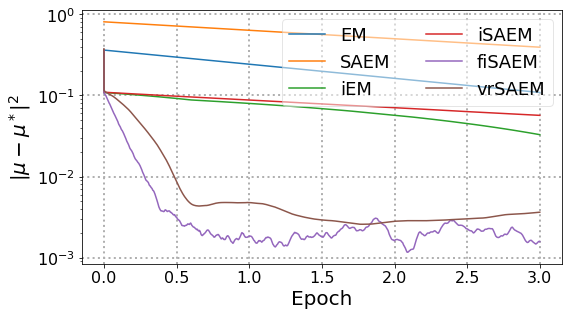
\includegraphics[width=2.5in]{fig/tts_gmm_n100k.png}
\includegraphics[width=2.5in]{fig/figgmm.eps}
\end{center}
\caption{Precision $|\mu^{(k)} - \mu^*|^2$ per epoch\vspace{0.2in}}
\label{fig:gmm_tts}%\vspace{0.3in}
\end{figure}

We run the EM method until convergence (to double precision) to obtain the ML estimate $\mu^\star$ averaged on $50$ datasets. 
We compare the EM, iEM (incremental EM), SAEM, \ISAEM, \SAEMVR\ and \FISAEM\ methods in terms of their precision measured by $| \mu - \mu^\star |^2$. 
We set the stepsize of the \textsf{SA-step} for all method as $\gamma_k = 1/k^{\alpha}$ with $\alpha = 0.5$, and the stepsize $\rho_k$ for the \SAEMVR\ and the \FISAEM\ to a constant stepsize equal to $1/n^{2/3}$. 
The number of MC samples is fixed to $M=10$.
Figure~\ref{fig:gmm_tts} shows the precision $|\mu - \mu^*|^2$ for the different methods through the epoch(s) (one epoch equals $n$ iterations). 
The \SAEMVR\ and \FISAEM\ methods outperform the other stochastic methods, supporting the benefits of our scheme.

\vspace{0.08in}
\noindent \textbf{Model Assumptions:}
We use the GMM example to illustrate the required assumptions.

Many practical models can satisfy the compactness of the sets as in Assumption~A\ref{ass:compact}
For instance, the GMM example satisfies the conditions in \ref{ass:compact} as the sufficient statistics are composed of indicator functions and observations as defined Section~\ref{app:gmm_update} Equation~\eqref{eq:gmm_exp}.

Assumptions A\ref{ass:expected} and A\ref{ass:reg} are standard for the curved exponential family models.
For GMM, the following (strongly convex) regularization $\Pen( \param )$ ensures A\ref{ass:reg}:
$$
\Pen( \param ) = \frac{\delta}{2} \sum_{m=1}^M \mu_m^2 - \epsilon \sum_{m=1}^M  \log ( \omega_m )  - \epsilon \log \big( 1 - \sum_{m=1}^{M-1} \omega_m \big) \eqsp,
$$
since it ensures $\param^{(k)}$ is unique and lies in ${\rm int}( \Delta^M ) \times \rset^M$.
We remark that for A\ref{ass:expected}, it is possible to define the Lipschitz constant $\Lip{p}$ independently for each data $y_i$ to yield a refined characterization. 

Again, A\ref{ass:eigen} is satisfied by practical models. For GMM, it can be verified by deriving the closed form expression for $\operatorname{B}( \bss )$ and using A\ref{ass:compact}.

Under A\ref{ass:compact} and A\ref{ass:reg}, we have $\| \hat{\bm s}^{(k)} \| < \infty$ since $\Sset$ is compact and $\hat{\param}^{(k)} \in {\rm int}( \Param )$ for any $k \geq 0$ which thus ensure that the EM methods operate in a closed set throughout the optimization process.


\vspace{0.08in}
\noindent \textbf{Algorithms updates:}
In the sequel, recall that, for all $i \in \inter[n]$ and iteration $k$, the computed statistic $ \tilde{S}_{i_k}^{(k)}$ is defined by \eqref{eq:stat_gmm}.
At iteration $k$, the several E-steps defined by \eqref{eq:isaem} or \eqref{eq:vrsaem} and \eqref{eq:fisaem} leads to the definition of the quantity $\hat{\bss}^{(k+1)} $. For the GMM example, after the initialization of the quantity $\hat{\bss}^{(0)} = n^{-1} \sum\nolimits_{i=1}^n \overline{\bss}_i^{(0)} $, those E-steps break down as follows:


Define the the exact conditional expected value $\EE_{\param}[ 1_{\{z_i=m\}} | y= y_{i} ]$ as follows:
\beq \notag
\widetilde{\omega}_m ( y_{i} ; \param ) \eqdef \EE_{\param}[ 1_{\{z_i=m\}} | y= y_{i} ]
= \frac{ {\omega}_{m} \!~ {\rm exp}(-\frac{1}{2}( y_{i} - {\mu}_{i} )^2) }{  \sum_{j=1}^{M}{ {\omega}_{j} \!~ \exp(-\frac{1}{2}( y_{i} - {\mu}_{j} )^2)} } \eqsp,
\eeq


 \begin{protocol}[H]
  \floatname{algorithm}{Table}
\caption{Algorithms Updates}
  \begin{algorithmic}[1]
\STATE \textsf{Batch EM (EM)} \hspace{0.4cm} for all $i \in \inter$, compute $\overline{\bss}_{i}^{(k)}$ and set $$\hat{\bss}^{(k+1)} = n^{-1} \sum\nolimits_{i=1}^n \overline{\bss}_i^{(k)}$$
\STATE \textsf{Incremental EM (iEM)} \hspace{0.4cm} draw  $i_k$ uniformly at random on $\inter[n]$, compute $\overline{\bss}_{i_k}^{(k)}$ and set $$\hat{\bss}^{(k+1)} = n^{-1} \sum\nolimits_{i=1}^n \overline{\bss}_i^{(k)}$$
\STATE \textsf{Batch SAEM (SAEM)} \hspace{0.4cm} for all $i \in \inter$ compute $ \tilde{S}_{i}^{(k)}$ \eqref{eq:stat_gmm} and set  $$\hat{\bss}^{(k+1)} = \hat{\bss}^{(k)}(1 - \gamma_{k+1}) + \gamma_{k+1}\stt^{(k)}$$
\STATE \textsf{Variance Reduced Two-Timescale EM (\SAEMVR)} \hspace{0.4cm} draw  $i_k$ uniformly at random on $\inter[n]$, compute $ \tilde{S}_{i_k}^{(k)}$ via \eqref{eq:stat_gmm} and set $$\hat{\bss}^{(k+1)} = \hat{\bss}^{(k)}(1 - \gamma_{k+1})+ \gamma_{k+1} \big(\stt^{(k)} (1 - \rho) + \rho (\tilde{S}^{(\ell(k))} +  \big( \tilde{S}_{i_k}^{(k)}  -\tilde{S}_{i_k}^{(\ell(k))}   \big)) \big) $$
\STATE \textsf{Fast Incremental Two-Timescale EM (\FISAEM)} \hspace{0.4cm} draw  $i_k$ uniformly at random on $\inter[n]$, compute $ \tilde{S}_{i_k}^{(k)}$ via \eqref{eq:stat_gmm} and set $$ \hat{\bss}^{(k+1)} = \hat{\bss}^{(k)}(1 - \gamma_{k+1})+ \gamma_{k+1} \big(\stt^{(k)} (1 - \rho) + \rho (\overline{\StocEstep}^{(k)} + \big( \tilde{S}_{i_k}^{(k)}  - \tilde{S}_{i_k}^{(t_{i_k}^k)}) \big) \eqsp.$$
  \end{algorithmic}
\end{protocol}


Finally, the $k$-th update reads $\hp{k+1} = \overline{\param} (\hat{\bss}^{(k+1)})$ where the function ${\bm s} \to \overline{\param}({\bm s})$ is defined by \eqref{eq:mstep_gmm}.


\subsection{Deformable Template Model for Image Analysis}


\vspace{0.08in}
\noindent \textbf{Model and EM Updates:} Let $(y_i, i \in \inter)$ be observed gray level images defined on a grid of pixels.
Let $u \in \mathcal{U} \subset \rset^2$ denote the pixel index on the image and $x_u \in \mathcal{D} \subset \rset^2$ its location.
The model used in this experiment suggests that each image $y_i$ is a deformation of a template, noted $I: \mathcal{D} \to \rset$, common to all images of the dataset:
\beq\label{eq:deformablemodel}
y_{i}(u)=I\left(x_{u}-\Phi_{i}\left(x_{u}, z_i\right)\right)+\varepsilon_{i}(u)
\eeq
where $\Phi_i: \rset^2 \to \rset^2$ is a deformation function, $z_i$ some latent variable parameterizing this deformation and $\varepsilon_{i} \sim \mathcal{N}(0,\sigma^2)$ is an observation error.
The template model, given $\{p_k\}_{k=1}^{k_p}$ landmarks on the template, a fixed known kernel $\mathbf{K}_{\mathbf{p}}$ and a vector of parameters $\beta \in \rset^{k_p}$ is defined as follows:
\beq\notag\label{eq:template}
I_{\xi}=\mathbf{K}_{\mathbf{p}} \beta, \quad \textrm{where} \quad \left(\mathbf{K}_{\mathbf{p}} \beta \right)(x)=\sum_{k=1}^{k_{p}} \mathbf{K}_{\mathbf{p}}\left(x, p_{k}\right) \beta_k\eqs.
\eeq
Given a set of landmarks $\{g_k\}_{k=1}^{k_g}$ and a fixed kernel $\mathbf{K}_{\mathbf{g}}$, we parameterize the deformation $\Phi_{i}$ as:
\beq\notag
\begin{split}
\Phi_{i}=\mathbf{K}_{\mathbf{g}} z_{i} \quad \textrm{where} \quad \left(\mathbf{K}_{\mathbf{g}} z_{i}\right)(x)=\sum_{k=1}^{k_{s}} \mathbf{K}_{\mathbf{g}}\left(x, g_{k}\right)\left(z_{i}^{(1)}(k), z_{i}^{(2)}(k)\right)\eqs,
\end{split}
\eeq
where we put a Gaussian prior on the latent variables, $z_i \sim \mathcal{N}(0,\Gamma)$ and $z_i \in \left( \rset^{k_g}\right)^2$.
The vector of parameters we estimate is thus $\param = \big( \beta, \Gamma, \sigma  \big)$.

The complete model belongs to the curved exponential family, see~\cite{allassonniere2007towards}, which vector of sufficient statistics $S = \big(S_1(z),S_2(z),S_3(z) \big)$ read:
\beq \label{eq:suffstat_deformable2}
\begin{split}
& S_1(z) = \frac{1}{n} \sum_{i=1}^nS_1(y_i, z_i)  = \frac{1}{n} \sum_{i=1}^n \left(\mathbf{K}_{p}^{z_{i}}\right)^\top y_{i} \eqsp,\\
& S_2(z) =\frac{1}{n} \sum_{i=1}^n S_2(y_i, z_i) = \frac{1}{n} \sum_{i=1}^n \left(\mathbf{K}_{p}^{z_{i}}\right)^\top\left(\mathbf{K}_{p}^{z_{i}}\right)\eqsp,\\
& S_3(z) =\frac{1}{n} \sum_{i=1}^n S_3(y_i, z_i)  = \frac{1}{n}  \sum_{i=1}^n  z_{i}^{t} z_{i} \eqsp,
\end{split}
\eeq
where for any pixel $u \in \rset^2$ and $j \in \llbracket 1, k_g \rrbracket$ we denote:
\beq\notag
\mathbf{K}_{p}^{z_{i}}(x_u,j) = \mathbf{K}_{p}^{z_{i}}(x_u - \phi_i(x_u,z_i), p_j)\eqsp.
\eeq
Finally, the Two-Timescale \textsf{M-step} yields the following parameter updates:
\beq
\bar{\param}(\hat{s}) 
= \left(
\begin{array}{c}
\beta(\hat{s}) =   \hat{s}_2^{-1}(z) \hat{s}_1(z)    \\
\Gamma(\hat{s}) = \frac{1}{n} \hat{s}_3(z)   \\
 \sigma(\hat{s}) =\beta(\hat{s})^\top  \hat{s}_2(z) \beta(\hat{s}) - 2\beta(\hat{s}) \hat{s}_1(z)
\end{array}
\right)\eqsp,
\eeq
where $\hat{s} = (\hat{s}_1(z),\hat{s}_2(z),\hat{s}_3(z))$ is the vector of statistics obtained via the \textsf{SA-step} \eqref{eq:rmstep} and using the MC approximation of the sufficient statistics $\big(S_1(z),S_2(z),S_3(z) \big)$ defined in \eqref{eq:suffstat_deformable2}.


%The complete model \eqref{eq:deformablemodel} belongs to the curved exponential family, see~\cite{allassonniere2007towards}, which vector of sufficient statistics for all $i \in \inter$ is defined by $S(y_i,z_i) = ( \mathbf{K}_{p,z_{i}}^\top y_{i}, \mathbf{K}_{p,z_{i}}^\top \mathbf{K}_{p,z_{i}},  z_{i}^{t} z_{i} )$ where we denote $\mathbf{K}_{p,z_{i}} = \mathbf{K}_{p,z_{i}}(x_u - \phi_i(x_u,z_i), p_j)$.
%Then, the two-timescale M-step \eqref{eq:mstep} yields the following parameter updates $\bar{\param}(\hat{s})= \left(
%\bm{\beta}(\hat{s}) =   \hat{s}_2^{-1}(z) \hat{s}_1(z), \bm{\Gamma}(\hat{s}) =  \hat{s}_3(z)/n, \bm{\sigma}(\hat{s}) =\bm{\beta}(\hat{s})^\top  \hat{s}_2(z) \bm{\beta}(\hat{s}) - 2\bm{\beta}(\hat{s}) \hat{s}_1(z) \right)$
%where $\hat{s} = (\hat{s}_1(z),\hat{s}_2(z),\hat{s}_3(z))$ is the vector of statistics obtained via update \eqref{eq:twolevels} in Algorithm~\ref{alg:ttsem}.


\begin{figure*}[ht]
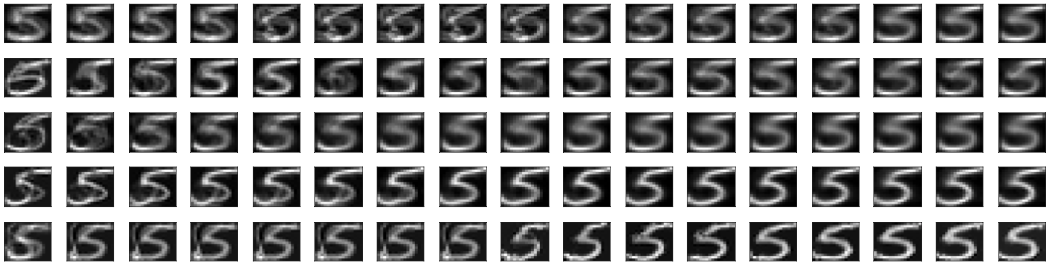
\includegraphics[width=\textwidth]{fig/deformable3}
\caption{(USPS Digits) Estimation of the template. From top to bottom: batch, online, \ISAEM,\ \SAEMVR\ and \FISAEM\ through 7 epochs. Note that Batch method templates are replicated in-between epochs for a fair comparison with incremental variants. }
\label{fig:results}
\end{figure*}


\vspace{0.08in}
\noindent \textbf{Numerical Experiment on US postal:} We apply model \eqref{eq:deformablemodel} and our Algorithm~\ref{alg:ttsem} to a collection of handwritten digits, called the US postal database~\cite{hull1994database}, featuring $n = 1\, 000$, $(16 \times 16)$-pixel images for each class of digits from $0$ to $9$.
The main challenge with this dataset stems from the geometric dispersion within each class of digit as shown Figure~\ref{fig:variancedigit} for digit $5$.
We thus ought to use our deformable template model~\eqref{eq:deformablemodel} in order to account for both sources of variability: the intrinsic template to each class of digit and the small and local deformations in each observed image.
\begin{figure}[H]

\includegraphics[width=\textwidth]{fig/variancedigit.png}
\caption{Training set of the USPS database (20 images for digit $5$)}
\label{fig:variancedigit}
\end{figure}

Figure~\ref{fig:results} shows the resulting synthetic images for digit $5$ through several epochs, for the batch method, the online SAEM, the incremental SAEM and the various two-timescale methods.
For all methods, the initialization of the template \eqref{eq:template} is the mean of the gray level images.
In our experiments, we have chosen Gaussian kernels for both, $\mathbf{K}_{\mathbf{p}}$ and $\mathbf{K}_{\mathbf{g}}$, defined on $\rset^2$ and centered on the landmark points$\{p_k\}_{k=1}^{k_p}$ and $\{g_k\}_{k=1}^{k_g}$ with standard respective standard deviations of $0.12$ and $0.3$. 
We set $k_p = 15$  and  $k_g = 6$ equidistributed landmarks points on the grid for the training procedure. 
The hyperparameters are kept the same and reads as follows $M = 400$, $ \gamma_k = 1/k^{0.6}$ and $ p = 16$.
The standard deviation of the measurement errors is set to $0.1$.
Those hyperparameters are inspired by relevant studies~\cite{allassonniere2008stochastic,allassonniere2010construction}.
For the simulation part, we use the Carlin and Chib MCMC procedure, see~\cite{carlin1995bayesian}, refer to~\cite{maire2016online} for more details.

In particular, the choice of the geometric covariance, indexed by $g$, in such study is critical since it has a direct impact on the \emph{sharpness} of the templates.
As for the photometric hyperparameter, indexed by $p$, both the template and the geometry are impacted, in the sense that with a large photometric variance, the kernel centered on one landmark \emph{spreads out} to many of its neighbors.


As the iterations proceed, the templates become sharper.
Figure~\ref{fig:results} displays the virtue of the \SAEMVR\ and \FISAEM\ methods that obtain a more \textit{contrasted} and \textit{accurate} template estimate. 
The incremental and online versions are better in the very first epochs compared to the batch method, given the high computational cost of the latter. 
After a few epochs, the batch SAEM estimates similar template as the incremental and online methods due to their high variance. 
Our variance reduced and fast incremental variants are effective in the long run and sharpen the template estimates contrasting between the background and the regions of interest in the image.

\subsection{Pharmacokinetics (PK) Model with Absorption Lag Time}
This numerical example was conducted in order to characterize the pharmacokinetics (PK) of orally administered drug to simulated patients, using a population pharmacokinetics approach. $M = 50$ synthetic datasets were generated for $n = 5000$ patients with $10$ observations (concentration measures) per patient.
The goal is to model the evolution of the concentration of the absorbed drug using a \emph{nonlinear} and \emph{latent} variable model. 

\vspace{0.08in}
\noindent \textbf{Model and Explicit Updates:}
We consider a one-compartment PK model for oral administration with an absorption lag-time ($T^{\textrm{lag}}$), assuming first-order absorption and linear elimination processes.
The final model includes the following variables: $ka$ the absorption rate constant, $V$ the volume of distribution, $k$ the elimination rate constant and $T^{\textrm{lag}}$ the absorption lag-time. 
We also add several covariates to our model such as $D$ the dose of drug administered, $t$ the time at which measures are taken and the weight of the patient influencing the volume $V$. More precisely, the log-volume $\log(V)$ is a linear function of the log-weight $lw70= \log(wt/70)$.
Let $ z_i=(T_i^{\textrm{lag}}, ka_i, V_i, k_i)$ be the vector of individual PK parameters, different for each individual $i$.
The final model reads:
\begin{equation} \label{eq:pkmodel}
\begin{split}
& y_{ij} = f(t_{ij},z_i)+ \varepsilon_{ij} \\
& \textrm{where} \quad f(t_{ij},z_i) = \frac{D\,ka_i}{V(ka_i - k_i)}(\exponential^{-ka_i\,(t_{ij} - T_i^{\textrm{lag}})}-\exponential^{-k_i\,(t_{ij} - T_i^{\textrm{lag}})})\eqs,
\end{split}
\end{equation}
where $y_{ij}$ is the $j$-th concentration measurement of the drug of dosage $D$ injected at time $t_{ij}$ for patient $i$.
We assume in this example that the residual errors $\varepsilon_{ij}$ are independent and normally distributed with mean 0 and variance $\sigma^2$.
Lognormal distributions are used for the four PK parameters:
\begin{align}
& \log(T_i^{\textrm{lag}}) \sim \mathcal{N}(\log(T^{\textrm{lag}}_{\rm pop}), \omega^2_{T^{\textrm{lag}}} ) \eqs, \log(ka_i) \sim \mathcal{N}(\log(ka_{\rm pop}), \omega^2_{ka})\eqs,\notag\\
&\log(V_i) \sim \mathcal{N}(\log(V_{\rm pop}), \omega^2_{V})\eqs,
 \log(k_i) \sim \mathcal{N}(\log(k_{\rm pop}), \omega^2_{k})\eqs.\notag
\end{align}
We note that the complete model $(y,z)$ defined by \eqref{eq:pkmodel} belongs to the curved exponential family, which vector of sufficient statistics $S = \big(S_1(z),S_2(z),S_3(z) \big)$ reads:
\beq \label{eq:suffstat_deformable3}
\begin{split}
S_1(z) & = \frac{1}{n} \sum_{i=1}^n z_i  \\
 S_2(z) &=\frac{1}{n} \sum_{i=1}^n z_i^\top z_i \\
 S_3(z)  &= \frac{1}{n}  \sum_{i=1}^n  \left(y_i - f(t_{i},z_i)\right)^2
\end{split}
\eeq
where we have noted $y_i$ and $t_i$ the vector of observations and time for each patient $i \in \inter$.
At iteration $k$, and setting the number of MC samples to $1$ for the sake of clarity, the MC sampling $z_i^{(k)} \sim p(z_i |y_i, \theta^{(k)})$ is performed using a Metropolis-Hastings procedure detailed in Appendix~\ref{app:experiments}. The quantities $\stt^{(k+1)}$ and $\hat{\bss}^{(k+1)}$ are then updated according to the different methods introduced in our paper, see Table~\ref{alg:prox}.
Finally the maximization step yields:
\beq \label{eq:mstep_pk}
\overline{\param} ( {\bm s} )
= \left(
\begin{array}{c}
\hat{\bss}^{(k+1)}_1 \\
\hat{\bss}^{(k+1)}_2 - \hat{\bss}^{(k+1)}_1 \left(\hat{\bss}^{(k+1)}_1 \right)^\top \vspace{.2cm} \\
\hat{\bss}^{(k+1)}_3
\end{array}
\right)
= \left(
\begin{array}{c}
\overline{\bm{z_{\rm pop}}} ( \hat{\bss}^{(k+1)}) \\
\overline{\bm{\omega_{z}}} ( \hat{\bss}^{(k+1)}) \\
\overline{\bm{\sigma}} ( \hat{\bss}^{(k+1)})
\end{array}
\right) \eqsp.
\eeq
where $z_{\rm pop}$ denotes the vector of fixed effects $(T^{\textrm{lag}}_{\rm pop}, ka_{\rm pop}, V_{\rm pop}, k_{\rm pop})$.

        
\begin{figure}
\begin{center}
%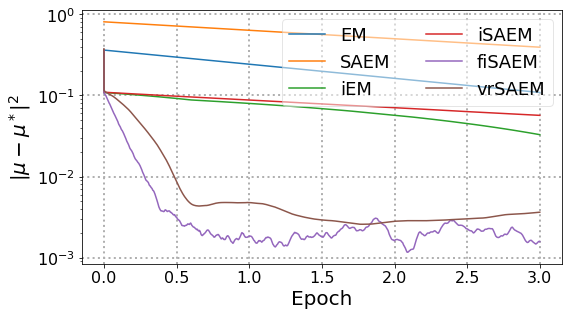
\includegraphics[width=2.5in]{fig/tts_gmm_n100k.png}
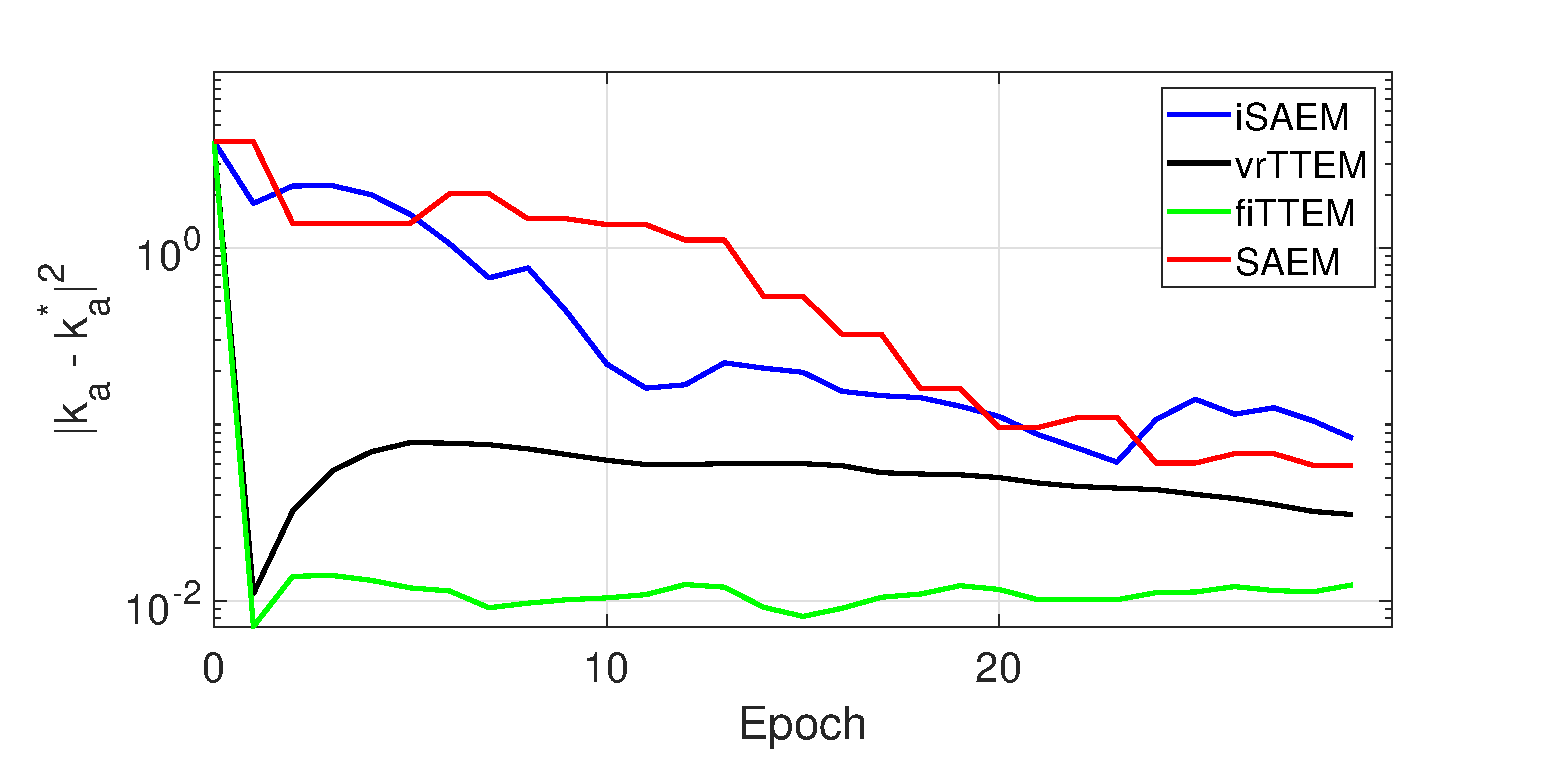
\includegraphics[width=4.9in]{fig/figpk.eps}
\end{center}
\caption{Precision $|ka^{(k)} - ka^*|^2$ per epoch}
\label{fig:pk_tts}
\end{figure}

\vspace{0.08in}
\noindent \textbf{Monte Carlo study:}
We conduct a Monte Carlo study to showcase the benefits of our scheme.
$M=50$ datasets have been simulated using the following PK parameters values:
$T^{\textrm{lag}}_{\rm pop} =1$, $ka_{\rm pop} =1$, $V_{\rm pop}= 8$, $k_{\rm pop}=0.1$, $ \omega_{T^{\textrm{lag}}}=0.4$, $\omega_{ka}=0.5$, $\omega_{V}=0.2$, $\omega_{k}=0.3$ and $\sigma^2=0.5$.
We define the mean square distance over the $M$ replicates $E_k(\ell) = \frac{1}{M}\sum_{m=1}^{M}{\left(\theta_k^{(m)}(\ell) - \theta^* \right)^2}$ and plot it against the epochs (passes over the data) in Figure~\ref{fig:pk_tts}.	
Note that the {\sf MC-step} \eqref{eq:mcstep} is performed using a Metropolis Hastings procedure since the posterior distribution under the model $\theta$ noted $p(z_i | y_i, \theta)$ is intractable, mainly due to the nonlinearity of the model \eqref{eq:pkmodel}.
Figure~\ref{fig:pk_tts} shows clear advantage of variance reduced methods (\SAEMVR\ and \FISAEM\ ) avoiding the twists and turns displayed by the incremental and the batch methods (iSAEM and SAEM).


\vspace{0.08in}
\noindent \textbf{Metropolis Hastings algorithm.}
During the simulation step of the MISSO method, the sampling from the target distribution $\pi(z_{i} , \param) \eqdef p(z_{i}|y_i ,\param)$ is performed using a Metropolis Hastings (MH) algorithm~\cite{meyn2012markov} with proposal distribution $q(z_{i}, \delta)$ where $\param = (z_{\rm pop}, \omega_{z})$ and $ \delta$ is the vector of parameters of the proposal distribution. Commonly they parameterize a Gaussian proposal.
The MH algorithm is summarized in~\ref{alg:mh}.

\begin{algorithm}[H]
\algsetup{indent=1em}
\begin{algorithmic}[1]
\STATE \textbf{Input:} initialization $z_{i,0} \sim q(z_{i}; {\bm \delta})$
\FOR {$m=1, \cdots ,M$}
\STATE Sample $z_{i,m} \sim q(z_{i}; {\bm \delta})$
\STATE Sample $u \sim \mathcal{U}(\llbracket 0, 1 \rrbracket)$
\STATE Calculate the ratio $r = \frac{\pi(z_{i,m}; \param)/q(z_{i,m}); {\bm \delta})}{\pi(z_{i,m-1}; \param)/q(z_{i,m-1}); {\bm \delta})}$
\IF{$u < r$}
\STATE Accept $z_{i,m}$
\ELSE
\STATE $z_{i,m} \leftarrow z_{i,m-1}$
\ENDIF
\ENDFOR
\STATE \textbf{Output:} $z_{i,M}$
\end{algorithmic}
\caption{MH aglorithm}
\label{alg:mh}
        \end{algorithm}




\section{Conclusion}


This paper introduces a new class of two-timescale EM methods for learning latent variable models.
In particular, the models dealt with in this paper belong to the curved exponential family and are possibly nonconvex.
The nonconvexity of the problem is tackled using a Robbins-Monro type of update, which represents the \textit{first level} of our class of methods.
The scalability with the number of samples is performed through a variance reduced and incremental update, the \textit{second} and last level of our newly introduced scheme.
The various algorithms are interpreted as scaled gradient methods, in the space of the sufficient statistics, and our convergence results are \emph{global}, in the sense of independence of the initial values, and \emph{non-asymptotic}, \ie true for any random termination number.
Numerical examples illustrate the benefits of our scheme on synthetic and real tasks.



% use section* for acknowledgment
%\section*{Acknowledgment}
%
%
%The authors would like to thank...


% Can use something like this to put references on a page
% by themselves when using endfloat and the captionsoff option.
\ifCLASSOPTIONcaptionsoff
  \newpage
\fi

\newpage





\newpage

\bibliographystyle{IEEEtran}
\bibliography{references}

\begin{IEEEbiography}{Belhal Karimi}
Biography text here.
\end{IEEEbiography}


\begin{IEEEbiography}{Ping Li}
Biography text here.
\end{IEEEbiography}


% You can push biographies down or up by placing
% a \vfill before or after them. The appropriate
% use of \vfill depends on what kind of text is
% on the last page and whether or not the columns
% are being equalized.

%\vfill

% Can be used to pull up biographies so that the bottom of the last one
% is flush with the other column.
%\enlargethispage{-5in}



% that's all folks

\newpage


\onecolumn 
\appendices


\section{Proofs for the \ISAEM\ Algorithm}
\subsection{Proof of Lemma~\ref{lem:growth}}\label{app:growth}
\begin{Lemma} 
Assume A\ref{ass:reg},A\ref{ass:eigen}. For all $\bss \in \Sset$,
\beq \label{eq:semigrad2}
\upsilon_{\min}^{-1} \pscal{\grd V ( {\bss} ) }{ {\bss} - \os( \op ({\bss})) }
\geq \| {\bss} - \os( \op ({\bss})) \|^2 \geq \upsilon_{\max}^{-2} \| \grd V ( {\bss} ) \|^2,
\eeq
\end{Lemma}
\begin{proof}
Using A\ref{ass:reg} and the fact that we can exchange integration with differentiation and the Fisher's identity,   we obtain
\beq \label{eq:grd_v}
\begin{split}
\grd_{ \bss} V( {\bss} ) & = \jacob{ \overline{\param} }{ \bss }{\bss}^\top
\Big( \grd_\param \Pen( \mstep{\bss} )  + \grd_\param \calL( \overline\param( {\bss} ) )  \Big) \\
& =  \jacob{ \overline{\param} }{ \bss }{\bss}^\top \Big( \grd_\param \psi( \mstep{\bss}) + \grd_\param \Pen( \mstep{\bss} ) - \jacob{\phi}{\param}{\mstep{\bss} }^\top  \os( \op ({\bss})) \Big)\\
& =   \jacob{ \overline{\param} }{ \bss }{\bss}^\top \jacob{\phi}{\param}{ \mstep{\bss} }^\top \!~ ({\bss} - \os( \op ({\bss})) ) \eqsp,
\end{split}
\eeq
Consider the following vector map:
\beq\notag
{\bss} \to \grd_{\param} L(\bss, \param) \vert_{\param= \mstep{\bss}}= \grd_\param \psi ( \mstep{\bss} ) + \grd_{ \param} \Pen(\mstep{\bss}  ) - \jacob{ \phi }{ \param }{\mstep{\bss}  }^\top \!~{\bss} \eqsp.
\eeq
Taking the gradient of the above map \wrt ${\bss}$ and using assumption A\ref{ass:reg}, we show that:
\beq\notag
{\bm 0} = - \jacob{\phi}{\param}{\mstep{\bss} } + \Big( \underbrace{ \grd_{\param}^2 \big( \psi( \param ) + \Pen( \param ) - \pscal{ \phi( \param ) }{ {\bss} } \big)}_{= \hess{{L}}{\param} ( {\bss}; \param )} \big|_{\param = \mstep{\bss}  } \Big) \jacob{ \overline{\param} }{\bss}{\bss} \eqsp.
\eeq
The above yields
\beq\notag
\grd_{ \bss} V( {\bss} )  = \operatorname{B}(\bss) ({\bss} - \os( \op ({\bss})) ) \eqsp,
\eeq
where we recall $\operatorname{B}(\bss) = \jacob{ \phi }{ \param }{ \mstep{\bss} } \Big( \hess{{L}}{\param}( {\bss}; \mstep{\bss} )  \Big)^{-1} \jacob{ \phi }{ \param }{\mstep{\bss} }^\top$. The proof of \eqref{eq:semigrad2} follows directly from the assumption~A\ref{ass:eigen}.
\end{proof}


%\section{Proof of Lemma~\ref{lem:meanfield_isaem}}\label{app:prooflemmainc}
\vspace{0.2in}

\subsection{Proof of Theorem~\ref{thm:isaem}}\label{app:theoremisaem}
Beforehand, We present two intermediary Lemmas important for the analysis of the incremental update of the iSAEM algorithm.
The first one gives a characterization of the quantity $\EE[\stt^{(k+1)} - \hat{\bss}^{(k)}]$:
\begin{Lemma}
 Assume A\ref{ass:compact}. The update \eqref{eq:isaem} is equivalent to the following update on the resulting statistics 
\beq\notag
\hat{\bss}^{(k+1)} =  \hat{\bss}^{(k)}  + \gamma_{k+1} \big( \stt^{(k+1)} - \hat{\bss}^{(k)} \big) \eqsp.
\eeq 
Also:
\beq\notag
\EE[\stt^{(k+1)} - \hat{\bss}^{(k)}] = \EE[\overline{\bss}^{(k)} - \hat{\bss}^{(k)}] + \left(1 - \frac{1}{n} \right) \EE\left[\frac{1}{n} \sum_{i=1}^n \tilde{S}_i^{(\tau_i^k)}- \overline{\bss}^{(k)}\right]  +\frac{1}{n}\EE[\eta_{i_k}^{(k+1)}]\eqsp ,
\eeq
where $\overline{\bss}^{(k)}$ is defined by \eqref{eq:definition-overline-bss} and $\tau_i^k = \max \{ k' : i_{k'} = i,~k' < k \}$.
\end{Lemma}
\begin{proof}
From update \eqref{eq:isaem}, we have:
\beq\notag
\begin{split}
\stt^{(k+1)} - \hat{\bss}^{(k)} & = \stt^{(k)} - \hat{\bss}^{(k)} +\frac{1}{n}\left( \tilde{S}_{i_k}^{(k+1)} - \tilde{S}_{i_k}^{(\tau_i^k)}  \right)\\
& = \overline{\bss}^{(k)} - \hat{\bss}^{(k)} + \stt^{(k)}- \overline{\bss}^{(k)}  - \frac{1}{n}\left( \tilde{S}_{i_k}^{(\tau_i^k)} - \tilde{S}_{i_k}^{(k+1)}   \right) \eqsp .
\end{split}
\eeq
Since $\tilde{S}_{i_k}^{(k+1)} = \overline{\bss}_{i_k}(\param^{(k)}) + \eta_{i_k}^{(k+1)}$ we have 
\beq\notag
\begin{split}
\stt^{(k+1)} - \hat{\bss}^{(k)} = \overline{\bss}^{(k)} - \hat{\bss}^{(k)} + \stt^{(k)}- \overline{\bss}^{(k)}  - \frac{1}{n}\left( \tilde{S}_{i_k}^{(\tau_i^k)} -  \overline{\bss}_{i_k}(\param^{(k)})   \right) + \frac{1}{n}\eta_{i_k}^{(k+1)}\eqsp .
\end{split}
\eeq
Taking the full expectation of both side of the equation leads to:
\beq\notag
\begin{split}
\EE[\stt^{(k+1)} - \hat{\bss}^{(k)}] = \EE[\overline{\bss}^{(k)} - \hat{\bss}^{(k)}] & + \EE\left[\frac{1}{n} \sum_{i=1}^n \tilde{S}_i^{(\tau_i^k)}-  \overline{\bss}^{(k)}\right] \\
& -\frac{1}{n} \EE[\EE[ \tilde{S}_i^{(\tau_i^k)}-  \overline{\bss}_{i_k}(\param^{(k)})  | \mathcal{F}_{k} ]] + \frac{1}{n} \EE[\eta_{i_k}^{(k+1)}] \eqsp.
\end{split}
\eeq
Since we have $\EE[ \tilde{S}_i^{(\tau_i^k)} | \mathcal{F}_{k} ] =\frac{1}{n} \sum_{i=1}^n \tilde{S}_i^{(\tau_i^k)}$ and $\EE\left[  \overline{\bss}_{i_k}(\param^{(k)})  | \mathcal{F}_{k} \right]= \overline{\bss}^{(k)}$, we conclude the proof of the Lemma.
\end{proof}

We also derived the following auxiliary Lemma which sets an upper bound for the quantity $\EE [ \|  \stt^{(k+1)} - \hs{k}   \|^2 ]$:
\begin{Lemma}\label{lem:aux2}
For any $k \geq 0$ and consider the \ISAEM\ update in \eqref{eq:isaem}, it holds that
\beq\notag
\begin{split}
\EE [ \|  \stt^{(k+1)} - \hs{k}   \|^2 ] \leq &4 \EE[ \|  \os^{(k)} - \hs{k} \|^2 ] 
+ \frac{2\Lip{\bss}^2}{n^3} \sum_{i=1}^n \EE\left[ \| \hs{k} - \hs{t_i^k} \|^2 \right]\\
&+ 2\frac{c_{\eta}}{M_k} + 4 \EE\left[\norm{ \frac{1}{n} \sum_{i=1}^n \tilde{S}_i^{(\tau_i^k)}-  \overline{\bss}^{(k)}}^2\right]  \eqsp.
\end{split}
\eeq
\end{Lemma}

\begin{proof}
Applying the \ISAEM\ update yields:
\beq\notag
\begin{split}
 \EE[ \|  \stt^{(k+1)} - \hs{k} \|^2 ]  =&  \EE[ \| \stt^{(k)} - \hs{k}  -\frac{1}{n}\big(\tilde{S}^{(\tau_i^k)}_{i_k} - \tilde{S}^{(k)}_{i_k}  \big)  \|^2 ]\\
 \leq  & 4 \EE\left[\norm{ \frac{1}{n} \sum_{i=1}^n \tilde{S}_i^{(\tau_i^k)}-  \overline{\bss}^{(k)}}^2\right] + 4 \EE[\|   \overline{\bss}^{(k)} - \hs{k} \|^2] \\
 &+  \frac{2}{n^2} \EE[ \| \os_{i_k}^{(k)} - \os_{i_k}^{(t_{i_k}^k)} \|^2] + 2\frac{c_{\eta}}{M_k} \eqsp.
\end{split}
\eeq

The last expectation can be further bounded by
\beq\notag
\begin{split}
&
\frac{2}{n^2}\EE[ \| \os_{i_k}^{(k)} - \os_{i_k}^{(t_{i_k}^k)} \|^2 ] = \frac{2}{n^3} \sum_{i=1}^n \EE[ \| \os_i^{(k)} - \os_i^{(t_i^k)} \|^2 ] \overset{(a)}{\leq} \frac{2\Lip{\bss}^2}{n^3}
\sum_{i=1}^n \EE[ \| \hs{k} - \hs{t_i^k} \|^2 ]\eqsp,
\end{split}
\eeq
where (a) is due to Lemma~\ref{lem:smooth} and which concludes the proof of the Lemma.

\end{proof}

\begin{Theorem}
Assume A\ref{ass:compact}-A\ref{ass:mcerror}.
Consider the \ISAEM\ sequence $\{\hat{\bss}^{(k)}\}_{k>0} \in \mathcal{S}$ obtained with $\rho_{k+1}=1$ for any $k \leq {\sf K}_{\sf m }$ where ${\sf K}_{\sf m }$ is a positive integer. 
Let $\{\gamma_{k} = 1/(k^a \alpha c_1 \overline{L})\}_{k>0}$, where $a \in (0,1)$, be a sequence of stepsizes, $c_1 = \upsilon_{\min}^{-1}$, $\alpha = \max\{8, 1+6\upsilon_{\min}\}$, $\overline{L} = \max\{ \Lip{\bss} , \Lip{V} \}$, $\beta = c_1 \overline{L}/n$. Then:
\beq\notag
\upsilon_{\max}^{-2}\sum_{k=0}^{{\sf K}_{\sf m }} \tilde{\alpha}_k \EE [\|\grd V( \hs{k} )\|^2]  \leq   \EE  [V( \hs{0} ) - V( \hs{{\sf K}_{\sf m }} ) ] + \sum_{k=0}^{{\sf K}_{\sf m }-1} \tilde{\Gamma}_k         \EE [\| \eta_{i_k}^{(k)}\|^2] \eqs.
\eeq
\end{Theorem} 

\begin{proof}

Under the smoothness of the Lyapunov function $V$ (cf. Lemma~\ref{lem:smooth}), we can write:
\beq\notag
\begin{split}
V( \hs{k+1} ) & \leq V( \hs{k} ) + \gamma_{k+1} \pscal{  \stt^{(k+1)}  - \hs{k}}{ \grd V( \hs{k} ) } + \frac{\gamma_{k+1}^2 \Lip{V}}{2} \|\stt^{(k+1)} -  \hs{k}  \|^2 \eqsp.\\
\end{split}
\eeq

Taking the expectation on both sides yields:
\beq\notag
\begin{split}
\EE \left[V( \hs{k+1} ) \right]  \leq \EE \left[ V( \hs{k} ) \right] & + \gamma_{k+1} \EE \left[\pscal{  \stt^{(k+1)}  - \hs{k}}{ \grd V( \hs{k} ) }  \right]\\
& + \frac{\gamma_{k+1}^2 \Lip{V}}{2} \EE \left[\|\stt^{(k+1)} -  \hs{k}  \|^2  \right]\eqsp.
\end{split}
\eeq

Using Lemma~\ref{lem:meanfield_isaem}, we obtain:
\beq\notag
\begin{split}
& \EE \left[\pscal{  \stt^{(k+1)}  - \hs{k}}{ \grd V( \hs{k} ) }  \right] \\
= &  \EE \left[\pscal{  \overline{\bss}^{(k)}  - \hs{k}}{ \grd V( \hs{k} ) }  \right]  + \left(1 - \frac{1}{n}\right)\EE\left[\pscal{ \frac{1}{n} \sum_{i=1}^n \tilde{S}_i^{(\tau_i^k)}-  \overline{\bss}^{(k)}}{ \grd V( \hs{k} ) }\right] \\
& +  \frac{1}{n} \EE \left[\pscal{ \eta_{i_k}^{(k)}}{ \grd V( \hs{k} ) }  \right]\\
 \overset{(a)}{\leq} & -\upsilon_{\min}\EE [\|  \overline{\bss}^{(k)}  - \hs{k}\|^2  ] + \left(1 - \frac{1}{n}\right)\EE\left[\pscal{ \frac{1}{n} \sum_{i=1}^n \tilde{S}_i^{(\tau_i^k)}-  \overline{\bss}^{(k)}}{ \grd V( \hs{k} ) }\right] \\
 & +  \frac{1}{n} \EE \left[\pscal{ \eta_{i_k}^{(k)}}{ \grd V( \hs{k} ) }  \right]\\
 \overset{(b)}{\leq} & -\upsilon_{\min}\EE [\|  \overline{\bss}^{(k)}  - \hs{k}\|^2  ] + \frac{1 - \frac{1}{n}}{2\beta}\EE\left[\norm{ \frac{1}{n} \sum_{i=1}^n \tilde{S}_i^{(\tau_i^k)}-  \overline{\bss}^{(k)}}^2\right]\\
& +  \frac{\beta(n-1) + 1}{2n}\EE\left[ \norm{\grd V( \hs{k} )}^2\right]  +  \frac{1}{2 n} \EE [\| \eta_{i_k}^{(k)}\|^2 ] \\
 \overset{(a)}{\leq} & \left(\upsilon^2_{\max}\frac{\beta(n-1) + 1}{2n}-\upsilon_{\min}\right) \EE [\|  \overline{\bss}^{(k)}  - \hs{k}\|^2  ] + \frac{1 - \frac{1}{n}}{2\beta}\EE\left[\norm{ \frac{1}{n} \sum_{i=1}^n \tilde{S}_i^{(\tau_i^k)}-  \overline{\bss}^{(k)}}^2\right]\\
 & +  \frac{1}{2 n} \EE [\| \eta_{i_k}^{(k)}\|^2 ] \eqsp,
\end{split}
\eeq
where (a) is due to the growth condition \eqref{lem:growth} and (b) is due to Young's inequality (with $\beta \to 1$).
Note $a_k = \gamma_{k+1}\left(\upsilon_{\min} - \upsilon^2_{\max}\frac{\beta(n-1) + 1}{2n}\right) $ and
\beq\label{eq:final1}
\begin{split}
a_k \EE [\|  \overline{\bss}^{(k)}  - \hs{k}\|^2  ]  \leq & \EE \left[ V( \hs{k} ) - V( \hs{k+1} ) \right] + \frac{\gamma_{k+1}^2 \Lip{V}}{2} \EE \left[\|\stt^{(k+1)} -  \hs{k}  \|^2  \right]\\
&+ \frac{\gamma_{k+1}(1 - \frac{1}{n})}{2\beta}\EE\left[\norm{ \frac{1}{n} \sum_{i=1}^n \tilde{S}_i^{(\tau_i^k)}-  \overline{\bss}^{(k)}}^2\right]+  \frac{\gamma_{k+1}}{2 n} \EE [\| \eta_{i_k}^{(k)}\|^2 ] \eqsp.
\end{split}
\eeq

We now give an upper bound of $\EE \left[\|\stt^{(k+1)} -  \hs{k}  \|^2  \right]$ using Lemma~\ref{lem:aux2} and plug it into \eqref{eq:final1}:

\beq\label{eq:final2}
\begin{split}
& ( a_k - 2\gamma_{k+1}^2 \Lip{V} ) \EE [\|  \overline{\bss}^{(k)}  - \hs{k}\|^2 ]  \\
\leq &  \EE \left[ V( \hs{k} ) - V( \hs{k+1} ) \right] \\
&  +   \gamma_{k+1} \left(\frac{1}{2 \beta}(1 - \frac{1}{n} ) + 2 \gamma_{k+1}\Lip{V} \right)            \EE\left[\norm{ \frac{1}{n} \sum_{i=1}^n \tilde{S}_i^{(\tau_i^k)}-  \overline{\bss}^{(k)}}^2\right]\\
& + \gamma_{k+1} \left(\gamma_{k+1} \Lip{V} +    \frac{1}{2 n}\right)           \EE [\| \eta_{i_k}^{(k)}\|^2 ] \\
& + \frac{\gamma_{k+1}^2 \Lip{V}\Lip{\bss}^2}{n^3} \sum_{i=1}^n \EE[ \| \hs{k} - \hs{\tau_i^k} \|^2 ] \eqsp.
\end{split}
\eeq


Next, we observe that
\beq\notag
\frac{1}{n} \sum_{i=1}^n \EE[ \| \hs{k+1} - \hs{t_i^{k+1}} \|^2 ] = \frac{1}{n} \sum_{i=1}^n
\Big( \frac{1}{n} \EE[ \| \hs{k+1} - \hs{k} \|^2 ] + \frac{n-1}{n} \EE[ \| \hs{k+1} - \hs{\tau_i^k} \|^2 ]  \Big)\eqsp,
\eeq
where the equality holds as $i_k$ and $j_k$ are drawn independently. For any $\beta > 0$, it holds
\beq\notag
\begin{split}
& \EE[ \| \hs{k+1} - \hs{t_i^k} \|^2 ] \\
 =& \EE \Big[ \| \hs{k+1} - \hs{k} \|^2 + \| \hs{k} - \hs{\tau_i^k} \|^2 + 2 \pscal{\hs{k+1} - \hs{k}}{\hs{k}- \hs{\tau_i^k}} \Big] \\
=& \EE \Big[ \| \hs{k+1} - \hs{k} \|^2 + \| \hs{k} - \hs{\tau_i^k} \|^2 - 2 \gamma_{k+1} \pscal{ \hs{k} - \stt^{(k+1)} }{\hs{k}- \hs{\tau_i^k}} \Big] \\
\leq&  \EE \Big[ \| \hs{k+1} - \hs{k} \|^2 + \| \hs{k} - \hs{\tau_i^k} \|^2 +  \frac{\gamma_{k+1}}{\beta} \| \hs{k} - \stt^{(k+1)}\|^2 + \gamma_{k+1} \beta \| \hs{k}- \hs{\tau_i^k} \|^2 \Big]\eqsp,
\end{split}
\eeq
where the last inequality is due to Young's inequality. Subsequently, we have
\beq\notag
\begin{split}
 &\frac{1}{n} \sum_{i=1}^n \EE[ \| \hs{k+1} - \hs{\tau_i^{k+1}} \|^2 ] \\
 \leq & \EE[  \| \hs{k+1} - \hs{k} \|^2 ] + \frac{n-1}{n^2} \sum_{i=1}^n \EE \Big[ (1+\gamma_{k+1} \beta) \|  \hs{k} - \hs{\tau_i^k} \|^2  + \frac{\gamma_{k+1}}{\beta} \|  \hs{k} - \stt^{(k+1)} \|^2 \Big]\eqsp.
\end{split}
\eeq
Observe that $\hs{k+1} - \hs{k} = - \gamma_{k+1} ( \hs{k} - \stt^{(k+1)} )$. Applying Lemma~\ref{lem:aux2} yields
\beq\notag
\begin{split}
& \frac{1}{n} \sum_{i=1}^n \EE[ \| \hs{k+1} - \hs{\tau_i^{k+1}} \|^2 ] \\
 \leq &\big(\gamma_{k+1}^2 +\frac{n-1}{n}\frac{\gamma_{k+1}}{\beta}  \big)\EE \Big[  \|   \stt^{(k+1)} -  \hs{k} \|^2  \Big] + \sum_{i=1}^n \EE \Big[  \frac{1 - \frac{1}{n} + \gamma_{k+1} \beta}{n} \|  \hs{k} - \hs{\tau_i^k} \|^2  \Big] \\
 \leq & 4\big(\gamma_{k+1}^2 +\frac{\gamma_{k+1}}{\beta}  \big)\EE \Big[  \|   \os^{(k)} - \hs{k}  \|^2  \Big] + 2\big(\gamma_{k+1}^2 +\frac{\gamma_{k+1}}{\beta}  \big)\EE [\| \eta_{i_k}^{(k)}\|^2 ]\\
+&  4 \big(\gamma_{k+1}^2 +\frac{\gamma_{k+1}}{\beta}  \big)\EE\left[\norm{ \frac{1}{n} \sum_{i=1}^n \tilde{S}_i^{(\tau_i^k)}-  \overline{\bss}^{(k)}}^2\right] \\
+&  \sum_{i=1}^n \EE \Big[ \frac{1 - \frac{1}{n} + \gamma_{k+1} \beta + \frac{2\gamma_{k+1} \Lip{\bss}^2}{n^2}(\gamma_{k+1} +\frac{1}{\beta})}{n} \|  \hs{k} - \hs{t_i^k} \|^2  \Big]  \eqsp.
\end{split}
\eeq
Let us define
\beq\notag
\Delta^{(k)} \eqdef \frac{1}{n} \sum_{i=1}^n \EE[ \| \hs{k} - \hs{\tau_i^{k}} \|^2 ]\eqsp.
\eeq
From the above, we get
\beq\notag
\begin{split}
 \Delta^{(k+1)} & \leq  \big(1 - \frac{1}{n} + \gamma_{k+1} \beta + \frac{2\gamma_{k+1} \Lip{\bss}^2}{n^2}(\gamma_{k+1} +\frac{1}{\beta})  \big) \Delta^{(k)} +4 \big(\gamma_{k+1}^2 +\frac{\gamma_{k+1}}{\beta}  \big) \EE \Big[  \|   \os^{(k)} - \hs{k}  \|^2  \Big]\\
 &  + 2\big(\gamma_{k+1}^2  +\frac{\gamma_{k+1}}{\beta}  \big)\EE [\| \eta_{i_k}^{(k)}\|^2 ]+  4 \big(\gamma_{k+1}^2 +\frac{\gamma_{k+1}}{\beta}  \big) \EE\left[\norm{ \frac{1}{n} \sum_{i=1}^n \tilde{S}_i^{(\tau_i^k)}-  \overline{\bss}^{(k)}}^2\right]\eqsp.
\end{split}
\eeq

Setting $c_1 = \upsilon_{\min}^{-1}$, $\alpha =\max\{8, 1+6\upsilon_{\min}\}$, $\overline{L} = \max\{ \Lip{\bss} , \Lip{V} \}$, $\gamma_{k+1} = \frac{1}{k \alpha c_1 \overline{L}}$, $\beta = \frac{c_1 \overline{L}}{n}$, $c_1(k\alpha-1) \geq c_1(\alpha-1) \geq 6$, $\alpha \geq 8$, we observe that
\beq\notag
1 - \frac{1}{n} + \gamma_{k+1} \beta + \frac{2\gamma_{k+1} \Lip{\bss}^2}{n^2}(\gamma_{k+1} +\frac{1}{\beta}) 
 \leq 1 - \frac{c_1(k\alpha  - 1) - 4}{k\alpha n c_1 } \leq 1 - \frac{2}{k\alpha n c_1 }\eqsp,
\eeq
which shows that $1 - \frac{1}{n} + \gamma_{k+1} \beta + \frac{2\gamma_{k+1} \Lip{\bss}^2}{n^2}(\gamma_{k+1} +\frac{1}{\beta})  \in (0,1)$ for any $k >0$.
Denote $ \Lambda_{(k+1)} =\frac{1}{n} - \gamma_{k+1} \beta - \frac{2\gamma_{k+1} \Lip{\bss}^2}{n^2}(\gamma_{k+1} +\frac{1}{\beta}) $ and note that $\Delta^{(0)} = 0$, thus the telescoping sum yields:
\beq\notag
\begin{split}
\Delta^{(k+1)} & \leq  4 \sum_{ \ell = 0 }^k \prod_{j = \ell +1}^k \Big( 1 -  \Lambda_{(j)} \Big) \big(\gamma_{\ell+1}^2 +\frac{\gamma_{\ell+1}}{\beta}  \big)  \EE[  \|  \os^{(\ell)} - \hs{\ell}  \|^2 ] \\
&+ 2\sum_{ \ell = 0 }^k \prod_{j = \ell +1}^k \Big( 1 -  \Lambda_{(j)} \Big) \big(\gamma_{\ell+1}^2  +\frac{\gamma_{\ell+1}}{\beta}  \big) \EE \left[\norm{ \eta_{i_\ell}^{(\ell)}}^2 \right]\\
& +  4 \sum_{ \ell = 0 }^k   \prod_{j = \ell +1}^k \Big( 1 -  \Lambda_{(j)} \Big)  \big(\gamma_{\ell+1}^2\\
&  +\frac{\gamma_{\ell+1}}{\beta}  \big)  \EE\left[\norm{ \frac{1}{n} \sum_{i=1}^n \tilde{S}_i^{(\tau_i^\ell)}-  \overline{\bss}^{(\ell)}}^2\right]\eqsp.
\end{split}
\eeq
Note $\omega_{k,\ell} = \prod_{j = \ell +1}^k \Big( 1 -  \Lambda_{(j)} \Big)$
Summing on both sides over $k=0$ to $k = {\sf K}_{\sf m }-1$ yields:

\beq\label{eq:Delta}
\begin{split}
& \sum_{k=0}^{{\sf K}_{\sf m }-1} \Delta^{(k+1)}\\
=&  4 \sum_{k=0}^{{\sf K}_{\sf m }-1} \big(\gamma_{k+1}^2 +\frac{\gamma_{k+1}}{\beta}  \big) \omega_{k,1} \EE[  \|  \os^{(k)} - \hs{k}  \|^2 ] + 2 \sum_{k=0}^{{\sf K}_{\sf m }-1} \big(\gamma_{k+1}^2  +\frac{\gamma_{k+1}}{\beta}  \big)\omega_{k,1}\EE \left[\norm{ \eta_{i_\ell}^{(k)}}^2 \right]\\
+ &  \sum_{k=0}^{{\sf K}_{\sf m }-1} 4 \big(\gamma_{k+1}^2 +\frac{\gamma_{k+1}}{\beta}  \big) \omega_{k,1}  \EE\left[\norm{ \frac{1}{n} \sum_{i=1}^n \tilde{S}_i^{(\tau_i^k)}-  \overline{\bss}^{(k)}}^2\right]\\
\leq &   \sum_{k=0}^{{\sf K}_{\sf m }-1}\frac{4\big(\gamma_{k+1}^2 +\frac{\gamma_{k+1}}{\beta}  \big)}{ \Lambda_{(k+1)}}   \EE[  \|  \os^{(k)} - \hs{k}  \|^2 ] + \sum_{k=0}^{{\sf K}_{\sf m }-1}\frac{2\big(\gamma_{k+1}^2 +\frac{\gamma_{k+1}}{\beta}  \big)}{ \Lambda_{(k+1)}}  \EE \left[\norm{ \eta_{i_\ell}^{(k)}}^2 \right]\\
 +&  \sum_{k=0}^{{\sf K}_{\sf m }-1}\frac{4\big(\gamma_{k+1}^2 +\frac{\gamma_{k+1}}{\beta}  \big)}{ \Lambda_{(k+1)}}  \EE\left[\norm{ \frac{1}{n} \sum_{i=1}^n \tilde{S}_i^{(\tau_i^k)}-  \overline{\bss}^{(k)}}^2\right]\eqsp.
\end{split}
\eeq
We recall \eqref{eq:final2} where we have summed on both sides from $k=0$ to $k = {\sf K}_{\sf m }-1$:
\beq\label{eq:final3}
\begin{split}
&\sum_{k=0}^{{\sf K}_{\sf m }-1}  \left( a_k - 2\gamma_{k+1}^2 \Lip{V} \right) \EE [\|  \overline{\bss}^{(k)}  - \hs{k}\|^2  ] \\
 \leq &  \EE \left[ V( \hs{0} ) - V( \hs{K} ) \right] \\
+&  \sum_{k=0}^{{\sf K}_{\sf m }-1} \gamma_{k+1} \left(\frac{1}{2 \beta}(1 - \frac{1}{n} ) + 2 \gamma_{k+1}\Lip{V} \right)            \EE\left[\norm{ \frac{1}{n} \sum_{i=1}^n \tilde{S}_i^{(\tau_i^k)}-  \overline{\bss}^{(k)}}^2\right]\\
+& \sum_{k=0}^{{\sf K}_{\sf m }-1} \gamma_{k+1} \left(\gamma_{k+1} \Lip{V} +    \frac{1}{2 n}\right)           \EE [\| \eta_{i_k}^{(k)}\|^2 ] \\
+& \sum_{k=0}^{{\sf K}_{\sf m }-1} \frac{\gamma_{k+1}^2 \Lip{V}\Lip{\bss}^2}{n^2} \Delta^{(k)}\eqsp.
\end{split}
\eeq
Plugging \eqref{eq:Delta} into \eqref{eq:final3} results in:
\beq\notag
\begin{split}
&\sum_{k=0}^{{\sf K}_{\sf m }-1}  \tilde{\alpha}_k \EE [\|  \overline{\bss}^{(k)}  - \hs{k}\|^2  ] + \sum_{k=0}^{{\sf K}_{\sf m }-1}  \tilde{\beta}_k \EE\left[\norm{ \frac{1}{n} \sum_{i=1}^n \tilde{S}_i^{(\tau_i^k)}-  \overline{\bss}^{(k)}}^2\right]\\
\leq  & \EE \left[ V( \hs{0} ) - V( \hs{K} ) \right]
+ \sum_{k=0}^{{\sf K}_{\sf m }-1} \tilde{\Gamma}_k         \EE [\| \eta_{i_k}^{(k)}\|^2 ] \eqsp,
\end{split}
\eeq
where
\begin{align*}
&  \tilde{\alpha}_k = a_k - 2\gamma_{k+1}^2 \Lip{V} -  \frac{\gamma_{k+1}^2 \Lip{V}\Lip{\bss}^2}{n^2}\frac{4\big(\gamma_{k+1}^2 +\frac{\gamma_{k+1}}{\beta}  \big)}{ \Lambda_{(k+1)}} \eqsp,  \\
&  \tilde{\beta}_k =  \gamma_{k+1} \left(\frac{1}{2 \beta}(1 - \frac{1}{n} ) + 2 \gamma_{k+1}\Lip{V} \right) -  \frac{\gamma_{k+1}^2 \Lip{V}\Lip{\bss}^2}{n^2}\frac{4\big(\gamma_{k+1}^2 +\frac{\gamma_{k+1}}{\beta}  \big)}{ \Lambda_{(k+1)}}\eqsp, \\
&  \tilde{\Gamma}_k = \gamma_{k+1} \left(\gamma_{k+1} \Lip{V} +    \frac{1}{2 n}\right)  +  \frac{\gamma_{k+1}^2 \Lip{V}\Lip{\bss}^2}{n^2} \frac{2\big(\gamma_{k+1}^2 +\frac{\gamma_{k+1}}{\beta}  \big)}{ \Lambda_{(k+1)}}\eqsp,
\end{align*}
and
\begin{align*}
&  a_k  = \gamma_{k+1}\left(\upsilon_{\min} - \upsilon^2_{\max}\frac{\beta(n-1) + 1}{2n}\right) \eqsp, \\
& \Lambda_{(k+1)} =\frac{1}{n} - \gamma_{k+1} \beta - \frac{2\gamma_{k+1} \Lip{\bss}^2}{n^2}(\gamma_{k+1} +\frac{1}{\beta})\eqsp, \\
& c_1 = \upsilon_{\min}^{-1}, \alpha = \max\{8, 1+6\upsilon_{\min}\}, \overline{L} = \max\{ \Lip{\bss} , \Lip{V} \}, \gamma_{k+1} = \frac{1}{k \alpha c_1 \overline{L}}, \beta = \frac{c_1 \overline{L}}{n}\eqsp.
\end{align*}
When, for any $k >0$, $\tilde{\alpha}_k \geq 0$, we have by Lemma~\ref{lem:growth} that:
\beq\notag
\sum_{k=0}^{{\sf K}_{\sf m }} \tilde{\alpha}_k \EE [\| \grd V( \hs{k} )\|^2 ] \leq \upsilon_{\max}^2\sum_{k=0}^{{\sf K}_{\sf m }} \tilde{\alpha}_k \EE [\|  \overline{\bss}^{(k)}  - \hs{k}\|^2  ]  \eqsp,
\eeq
which yields an upper bound of the gradient of the Lyapunov function $V$ along the path of the \ISAEM\ update and concludes the proof of the Theorem.
\end{proof}

\vspace{0.2in}

\section{Proofs for the \SAEMVR\ and the \FISAEM\ Algorithms}
\subsection{Proofs of Auxiliary Lemmas ( Lemma~\ref{lem:auxvrsaem}, Lemma~\ref{lem:aux1} and Lemma~\ref{lem:gap_dynamics})} \label{app:bothauxvrsaem}
\begin{Lemma}
Consider the \SAEMVR\ update~\eqref{eq:vrsaem} with $\rho_k = \rho$, it holds for all $k>0$ 
\beq\notag
\begin{split}
  \EE [\| \hs{k} - \stt^{(k+1)}\|^2 ] \leq& 2\rho^2 \EE[ \| \hs{k} - \os^{(k)} \|^2] +  2\rho^2\Lip{\bss}^2 \EE[ \| \hs{k} - \hs{\ell(k)} \|^2 ]\\
  &+2(1-\rho)^2 \EE[ \| \hs{(k)} - \stt^{(k)} \|^2 ]+ 2\rho^2\EE[\|\eta_{i_k}^{(k+1)} \|^2]\eqs,
\end{split}
\eeq
where we recall that $\ell(k)$ is the first iteration number in the epoch that iteration $k$ is in.
\end{Lemma}
\begin{proof}
Beforehand, we provide a rewiriting of the quantity $ \hs{k+1} - \hs{k} $ that will be useful throughout this proof:
\beq\label{eq:vrsaem_drift}
\begin{split}
\hs{k+1} - \hs{k} & = -\gamma_{k+1}  ( \hs{k} - \stt^{(k+1)}) \\
&=-\gamma_{k+1}  ( \hs{k} - (1-\rho)\stt^{(k)} - \rho\StocEstep^{(k+1)})\\
& = -\gamma_{k+1} \left((1-\rho)\left[\hs{k} - \stt^{(k)} \right] +\rho\left[\hs{k} - \StocEstep^{(k+1)}\right] \right) \eqsp.
\end{split}
\eeq
We observe, using the identity \eqref{eq:vrsaem_drift}, that
\beq \label{eq:auxlemvrsaem}
\EE[ \| \hs{k} -\stt^{(k+1)} \|^2 ] \leq 2\rho^2 \EE[ \| \hs{k} - \os^{(k)} \|^2] + 2\rho^2 \EE[ \| \os^{(k)} - \StocEstep^{(k+1)} \|^2 ]+ 2(1-\rho)^2 \EE[ \| \hs{(k)} - \stt^{(k)} \|^2 ].
\eeq
For the latter term, we obtain its upper bound as % note $\EE[\StocEstep^{(k+1)}] = \os^{(k)}$
\beq\notag
\begin{split}
&\EE[ \| \os^{(k)} - \StocEstep^{(k+1)} \|^2 ] \\
 = &\EE\Big[ \| \frac{1}{n} \sum_{i=1}^n \big( \os_i^{(k)} - \tilde{S}_i^{\ell(k)} \big) - \big( \os_{i_k}^{(k)} - \tilde{S}_{i_k}^{(\ell(k))} \big) \|^2 \Big] \\
 \overset{(a)}{\leq} & \EE[ \| \os_{i_k}^{(k)} - \os_{i_k}^{(\ell(k))} \|^2 ] + \EE[\|\eta_{i_k}^{(k+1)} \|^2] \overset{(b)}{\leq}  \Lip{\bss}^2 \EE[ \| \hs{k} - \hs{\ell(k)} \|^2 ]+ \EE[\|\eta_{i_k}^{(k+1)} \|^2]\eqsp,
\end{split}
\eeq
where $(a)$ uses the variance inequality and $(b)$ uses Lemma~\ref{lem:smooth}. 
Substituting into \eqref{eq:auxlemvrsaem} proves the lemma.
\end{proof}
\begin{Lemma}
Consider the \FISAEM\ update~\eqref{eq:fisaem} with $\rho_k = \rho$. It holds for all $k>0$ that
\beq\notag
\begin{split}
  \EE [\| \hs{k} - \stt^{(k+1)}\|^2 ] \leq& 2\rho^2 \EE[ \| \hs{k} - \os^{(k)} \|^2] +  2\rho^2\frac{\Lip{\bss}^2}{n}
\sum_{i=1}^n \EE[ \| \hs{k} - \hs{t_i^k} \|^2 ]\\
  &+2(1-\rho)^2 \EE[ \| \hs{(k)} - \stt^{(k)} \|^2 ]+ 2\rho^2\EE[\|\eta_{i_k}^{(k+1)} \|^2]\eqsp,
\end{split}
\eeq
where $\Lip{\bss}$ is the smoothness constant defined in Lemma~\ref{lem:smooth}.
\end{Lemma}

\begin{proof}
Beforehand, we provide a rewiriting of the quantity $ \hs{k+1} - \hs{k} $ that will be useful throughout this proof:
\beq\label{eq:fisaem_drift}
\begin{split}
\hs{k+1} - \hs{k}  & = -\gamma_{k+1}  ( \hs{k} - \stt^{(k+1)}) \\
& =-\gamma_{k+1}  ( \hs{k} - (1-\rho)\stt^{(k)} - \rho\StocEstep^{(k+1)})\\
& = -\gamma_{k+1} \left((1-\rho)\left[\hs{k} - \stt^{(k)} \right] +\rho\left[\hs{k} - \StocEstep^{(k+1)}\right] \right)\\
& =  -\gamma_{k+1} \left((1-\rho)\left[\hs{k} - \stt^{(k)} \right] +\rho\left[\hs{k} - \overline{\StocEstep}^{(k)} - \big( \tilde{S}_{i_k}^{(k)}  -  \tilde{S}_{i_k}^{(t_{i_k}^k)}  \big)\right] \right) \eqsp.
\end{split}
\eeq

We observe, using the identity \eqref{eq:fisaem_drift}, that
\beq \label{eq:auxlemfisaem}
\EE[ \| \hs{k} -\stt^{(k+1)} \|^2 ] \leq 2\rho^2 \EE[ \| \hs{k} - \os^{(k)} \|^2] + 2\rho^2 \EE[ \| \os^{(k)} - \StocEstep^{(k+1)} \|^2 ]+ 2(1-\rho)^2 \EE[ \| \hs{(k)} - \stt^{(k)} \|^2 ]\eqsp.
\eeq
For the latter term, we obtain its upper bound as % note $\EE[\StocEstep^{(k+1)}] = \os^{(k)}$
\beq\notag
\begin{split}
\EE[ \| \os^{(k)} - \StocEstep^{(k+1)} \|^2 ] & = \EE\Big[ \| \frac{1}{n} \sum_{i=1}^n \big( \os_i^{(k)} -\overline{\StocEstep}_i^{(k)} \big) - \big( \tilde{S}_{i_k}^{(k)} - \tilde{S}_{i_k}^{(t_{i_k}^k)} \big) \|^2 \Big] \\
& \overset{(a)}{\leq} \EE[ \| \os_{i_k}^{(k)} - \os_{i_k}^{(\ell(k))} \|^2 ] + \EE[\|\eta_{i_k}^{(k+1)} \|^2] \eqsp,
\end{split}
\eeq
where $(a)$ uses the variance inequality.
We can further bound the last expectation using Lemma~\ref{lem:smooth}:
\beq\notag
\EE[ \| \os_{i_k}^{(k)} - \os_{i_k}^{(t_{i_k}^k)} \|^2 ] = \frac{1}{n} \sum_{i=1}^n \EE[ \| \os_i^{(k)} - \os_i^{(t_i^k)} \|^2 ] \overset{(a)}{\leq} \frac{\Lip{\bss}^2}{n}
\sum_{i=1}^n \EE[ \| \hs{k} - \hs{t_i^k} \|^2 ]\eqsp.
\eeq
Substituting into \eqref{eq:auxlemfisaem} proves the lemma.
\end{proof}

\begin{Lemma} 
Considering a decreasing stepsize $\gamma_k \in (0,1)$ and a constant $\rho \in (0,1)$, we have
\beq\notag
\begin{split}
\EE [\| \hs{k} - \stt^{(k)}   \|^2]  \leq \frac{\rho}{1-\rho}\sum_{\ell = 0}^k (1-\gamma_{\ell} )^2 (   \StocEstep^{(\ell)} - \tilde{S}^{(\ell)})\eqs,
\end{split}
\eeq
where $\StocEstep^{(k)}  $ is defined either by Line~\ref{eq:vrsaem} (\SAEMVR\ ) or Line~\ref{eq:fisaem} (\FISAEM\ ).
\end{Lemma}
\begin{proof}
We begin by writing the two-timescale update:
\beq\label{eq:updatetwo}
\begin{split}
& \stt^{(k+1)} = \stt^{(k)} + \rho \big( \StocEstep^{(k+1)}- \stt^{(k)}  \big)\eqsp,\\
&  \hat{\bss}^{(k+1)} =  \hat{\bss}^{(k)}  + \gamma_{k+1}(\stt^{(k+1)} - \hat{\bss}^{(k)} ) \eqsp,
\end{split}
\eeq
where $\StocEstep^{(k+1)} = \frac{1}{n}\sum_{i=1}^n \tilde{S}_i^{(t_i^k)} + \big( \tilde{S}_{i_k}^{(k)}  - \tilde{S}_{i_k}^{(t_{i_k}^k)} \big) $ according to \eqref{eq:fisaem}.
Denote $\delta^{(k+1)} =  \hs{k+1} - \stt^{(k+1)} $. 
Then from \eqref{eq:updatetwo}, doing the subtraction of both equations yields:
\beq\notag
\delta^{(k+1)} = (1-\gamma_{k+1} ) \delta^{(k)} + \frac{\rho}{1-\rho}(1-\gamma_{k+1} )(  \StocEstep^{(k+1)} -  \stt^{(k+1)})\eqsp.
\eeq
Using the telescoping sum and noting that $\delta^{(0)} = 0$, we have
\beq\notag
\delta^{(k+1)} \leq \frac{\rho}{1-\rho}\sum_{\ell = 0}^k (1-\gamma_{\ell+1} )^2 (   \StocEstep^{(\ell+1)} - \tilde{S}^{(\ell+1)} )\eqsp.
\eeq 
\end{proof}


\subsection{Additional Intermediary Result}
\begin{Lemma} \label{lem:drift_fisaem}
 At iteration $k+1$,the drift term of update \eqref{eq:fisaem}, with $\rho_{k+1} = \rho$, is equivalent to the following :
\beq\notag
\begin{split}
 \hs{k} -  \stt^{(k+1)}= & \rho (\hs{k} - \overline{\bss}^{(k)})  + \rho \eta_{i_k}^{(k+1)}+ \rho \left[\big(\overline{\bss}_{i_k}^{(k)} - \tilde{S}_{i_k}^{(t_{i_k}^k)}\big) - \EE[\overline{\bss}_{i_k}^{(k)} - \tilde{S}_{i_k}^{(t_{i_k}^k)}] \right] \\
 &+ (1-\rho)\left( \hs{k} - \tilde{S}^{(k)}\right)\eqsp,
\end{split}
\eeq
where we recall that $\eta_{i_k}^{(k+1)}$, defined in \eqref{eq:mcerror}, which is the gap between the MC approximation and the expected statistics.
\end{Lemma}
\begin{proof}
Using the \FISAEM\ update $ \stt^{(k+1)} = (1 - \rho)\stt^{(k)} + \rho \StocEstep^{(k+1)}$ where $\StocEstep^{(k+1)} = \overline{\StocEstep}^{(k)} + \big( \tilde{S}_{i_k}^{(k)}  - \tilde{S}_{i_k}^{(t_{i_k}^k)} \big)$ leads to the following decomposition:
\beq\notag
\begin{split}
 & \stt^{(k+1)} - \hs{k} \\
 =& (1 - \rho)\stt^{(k)} + \rho \left( \overline{\StocEstep}^{(k)} + \big( \tilde{S}_{i_k}^{(k)}  - \tilde{S}_{i_k}^{(t_{i_k}^k)} \big) \right) - \hs{k}+\rho \overline{\bss}^{(k)} - \rho \overline{\bss}^{(k)} \\
 =& \rho (\overline{\bss}^{(k)} - \hs{k}) + \rho(\tilde{S}_{i_k}^{(k)} - \overline{\bss}^{(k)}_{i_k}) + (1-\rho)\left(\stt^{(k)} - \hs{k}\right) + \rho \left( \overline{\StocEstep}^{(k)} - \overline{\bss}^{(k)}+ \big( \overline{\bss}_{i_k}^{(k)}   - \tilde{S}_{i_k}^{(t_{i_k}^k)} \big) \right)\\ 
 =& \rho (\overline{\bss}^{(k)}-\hs{k}) + \rho \eta_{i_k}^{(k+1)} - \rho \left[\big(\overline{\bss}_{i_k}^{(k)} - \tilde{S}_{i_k}^{(t_{i_k}^k)}\big) - \EE[\overline{\bss}_{i_k}^{(k)} - \tilde{S}_{i_k}^{(t_{i_k}^k)}] \right] \\
 +& (1-\rho)\left(\stt^{(k)} - \hs{k}\right) \eqsp,
\end{split}
\eeq
where we observe that $\EE[\overline{\bss}_{i_k}^{(k)} - \tilde{S}_{i_k}^{(t_{i_k}^k)}] =\overline{\bss}^{(k)} -   \overline{\StocEstep}^{(k)} $ and which concludes the proof.

\textit{Important Note:} Note that $\overline{\bss}_{i_k}^{(k)} - \tilde{S}_{i_k}^{(t_{i_k}^k)}$ is not equal to $\eta_{i_k}^{(k+1)}$, defined in \eqref{eq:mcerror}, which is the gap between the MC approximation and the expected statistics. Indeed $\tilde{S}_{i_k}^{(t_{i_k}^k)}$ is not computed under the same model as $\overline{\bss}_{i_k}^{(k)}$.
\end{proof}


\subsection{Proof of Theorem~\ref{thm:vrsaem}}\label{app:theoremvrsaem}
\begin{Theorem}
Assume A\ref{ass:compact}-A\ref{ass:mcerror}.
Consider the \SAEMVR\ sequence $\{\hat{\bss}^{(k)}\}_{k>0} \in \mathcal{S}$ for any $k \leq {\sf K}_{\sf m }$ where ${\sf K}_{\sf m }$ is a positive integer. 
Let $\{\gamma_{k+1} = 1/(k^a \overline{L})\}_{k>0}$, where $a \in (0,1)$, be a sequence of stepsizes, $\overline{L} = \max \{\Lip{\bss}, \Lip{V} \}$, $\rho = \mu/( c_1 \overline{L}  n^{2/3})$, $m = n c_1^2/(2 \mu^2+\mu c_1^2)$ and a constant $\mu \in (0,1)$. Then:
\beq\notag
\EE[ \| \grd V( \hs{K} ) \|^2 ] \leq  \frac{2 n^{2/3} \overline{L}}{\mu {\sf P}_{\sf m} \upsilon_{\min}^2\upsilon_{\max}^2}\left( \EE[ \Delta V ]+  \sum_{k=0}^{{\sf K}_{\sf m }-1}  \tilde{\eta}^{(k+1)}\hspace{-0.1cm} + \chi^{(k+1)} \EE[\| \hs{k} - \tilde{S}^{(k)}\|^2]\right)  \eqsp.
\eeq
\end{Theorem} 

\begin{proof}

Using the smoothness of $V$ and update \eqref{eq:vrsaem}, we obtain:
\beq\label{eq:smoothvrsaem}
\begin{split}
V( \hs{k+1} ) & \leq V( \hs{k} ) + \pscal{  \hs{k+1} - \hs{k}  }{ \grd V( \hs{k} ) } + \frac{ \Lip{V}}{2} \| \hs{k+1} - \hs{k} \|^2\\
& \leq V( \hs{k} ) - \gamma_{k+1} \pscal{  \hs{k}-  \stt^{(k+1)} }{ \grd V( \hs{k} ) } + \frac{\gamma_{k+1}^2 \Lip{V}}{2} \|  \hs{k}  - \stt^{(k+1)} \|^2\eqsp.
\end{split}
\eeq
Denote $\Hdrift_{k+1} \eqdef  \hs{k} -  \stt^{(k+1)} $ the drift term of the \FISAEM\ update in \eqref{eq:rmstep} and  $\hmean_{k} =\hs{k} - \overline{\bss}^{(k)}$. Taking expectations on both sides show that
\beq \label{eq:lips_con}
\begin{split}
& \EE[ V( \hs{k+1} ) ] \\
 \overset{(a)}{\leq} &\EE[ V( \hs{k} ) ] - \gamma_{k+1}(1-\rho) \EE \Big[ \pscal{ \hs{k} - \stt^{(k)} }{\grd V( \hs{k} ) } \Big]\\
 &- \gamma_{k+1} \rho \EE \Big[ \pscal{ \hs{k} - \StocEstep^{(k+1)}  }{\grd V( \hs{k} ) } \Big]  +  \frac{\gamma_{k+1}^2 \Lip{V}}{2} \EE[ \| \Hdrift_{k+1} \|^2 ] \\
 \overset{(b)}{\leq}&  \EE[ V( \hs{k} ) ] - \gamma_{k+1} \rho \EE \Big[ \pscal{ \hmean_{k}  }{\grd V( \hs{k} ) } \Big]- \gamma_{k+1}(1-\rho) \EE \Big[ \pscal{ \hs{k} - \stt^{(k)} }{\grd V( \hs{k} ) } \Big] \\
  -&  \gamma_{k+1}\rho \EE \Big[ \pscal{ \eta_{i_k}^{(k+1)} }{\grd V( \hs{k} ) } \Big] + \frac{\gamma_{k+1}^2 \Lip{V}}{2} \EE[ \| \Hdrift_{k+1} \|^2 ] \\
 \overset{(c)}{\leq}&  \EE[ V( \hs{k} ) ] - \left(\gamma_{k+1} \rho \upsilon_{\min} + \gamma_{k+1}  \upsilon_{\max}^2 \right)  \EE \Big[ \norm{\hmean_{k}}^2 \Big]+ \frac{\gamma_{k+1}^2 \Lip{V}}{2} \EE[ \| \Hdrift_{k+1} \|^2 ]\\
 - &  \gamma_{k+1} \rho \EE\left[\norm{\eta_{i_k}^{(k+1)}}^2 \right] - \gamma_{k+1}(1-\rho) \EE \left[ \| \hs{k} - \tilde{S}^{(k)}\|^2 \right]  \eqsp,
\end{split}
\eeq
where we have used \eqref{eq:vrsaem_drift} in $(a)$ and $\EE \left[ \StocEstep^{(k+1)} \right] = \overline{\bss}^{(k)} + \EE[\eta_{i_k}^{(k+1)}]$ in $(b)$, the growth condition in Lemma~\ref{lem:growth} and Young's inequality with the constant equal to $1$ in $(c)$.

Furthermore, for $k+1 \leq \ell(k) + m$ (\ie $k+1$ is in the same epoch as $k$), we have
\beq\notag
\begin{split}
& \EE[ \| \hs{k+1} -  \hs{\ell(k)} \|^2 ] = \EE[ \| \hs{k+1} - \hs{k} + \hs{k} - \hs{\ell(k)} \|^2 ] \\
= & \EE \Big[  \| \hs{k} -  \hs{\ell(k)} \|^2 + \| \hs{k+1} - \hs{k}  \|^2 + 2 \pscal{\hs{k} -  \hs{\ell(k)} }{\hs{k+1} - \hs{k} } \Big] \\
= &  \EE \Big[ \| \hs{k} -  \hs{\ell(k)} \|^2 + \gamma_{k+1}^2 \| \Hdrift_{k+1} \|^2 \\
-&2\gamma_{k+1} \pscal{\hs{k} -  \hs{\ell(k)} }{ \rho(\hmean_{k} - \eta_{i_k}^{(k+1)}) + (1-\rho)( \hs{k} - \stt^{(k)} )  } \Big] \\
 \leq &\EE \Big[ (1 + \gamma_{k+1} \beta) \| \hs{k} -  \hs{\ell(k)} \|^2 + \gamma_{k+1}^2 \| \Hdrift_{k+1} \|^2 + \frac{\gamma_{k+1}\rho}{\beta} \| \hmean_{k} \|^2\\
 +  & \frac{\gamma_{k+1}\rho}{\beta} \|\eta_{i_k}^{(k+1)} \|^2 + \frac{\gamma_{k+1}(1-\rho)}{\beta} \| \hs{k} - \stt^{(k)} \|^2 \Big]\eqsp,
\end{split}
\eeq
where we first used \eqref{eq:vrsaem_drift} and the last inequality is due to Young's inequality.

Consider the following sequence
\beq\notag
R_k \eqdef \EE[ V( \hs{k} ) + b_{{k}} \| \hs{k} - \hs{\ell(k)} \|^2 ]\eqsp,
\eeq
where $b_k \eqdef \overline{b}_{k~{\rm mod}~m}$ is a periodic sequence where:
\beq\notag
\overline{b}_i = \overline{b}_{i+1} (1 + \gamma_{k+1} \beta + 2 \gamma_{k+1}^2\rho^2 \Lip{\bss}^2 ) + \gamma_{k+1}^2\rho^2 \Lip{V} \Lip{\bss}^2,~~i=0,1,\dots,m-1~~\text{with}~~\overline{b}_m = 0\eqsp.
\eeq
Note that $\overline{b}_i$ is decreasing with $i$ and this implies
\beq\notag
\overline{b}_i \leq \overline{b}_0 = \gamma_{k+1}^2\rho^2 \Lip{V} \Lip{\bss}^2 \frac{ (1 + \gamma_{k+1} \beta + 2 \gamma_{k+1}^2 \rho^2\Lip{\bss}^2 )^m - 1 }{ \gamma_{k+1} \beta + 2 \gamma_{k+1}^2 \rho^2\Lip{\bss}^2 },~i=1,2,\dots,m \eqsp.
\eeq
For $k+1 \leq \ell(k) + m$, we have the following inequality
\beq\notag
\begin{split}
R_{k+1 } & \leq  \EE \Big[ V( \hs{k} )  - \left(\gamma_{k+1} \rho \upsilon_{\min} + \gamma_{k+1}  \upsilon_{\max}^2 \right)  \| \hmean_{k} \|^2 + \frac{\gamma_{k+1}^2 \Lip{V}}{2} \| \Hdrift_{k+1}  \|^2 \Big] \\
& + \gamma_{k+1} \EE\left[\rho \norm{\eta_{i_k}^{(k+1)}}^2 -(1-\rho)\| \hs{k} - \tilde{S}^{(k)}\|^2 \right]\\
& + b_{k+1} \EE \left[ (1 + \gamma_{k+1} \beta) \| \hs{k} -  \hs{\ell(k)} \|^2 + \gamma_{k+1}^2 \| \Hdrift_{k+1} \|^2 + \frac{\gamma_{k+1}\rho}{\beta} \| \hmean_{k} \|^2 \right]\\
& + b_{k+1} \EE \left[ \frac{\gamma_{k+1}\rho}{\beta} \|\eta_{i_k}^{(k+1)} \|^2 + \frac{\gamma_{k+1}(1-\rho)}{\beta} \| \hs{k} - \stt^{(k)} \|^2 \right]\eqsp.
\end{split}
\eeq
And using Lemma~\ref{lem:auxvrsaem} we obtain:
\beq\notag
\begin{split}
& R_{k+1 }  \\
\leq & \EE \Big[ V( \hs{k} )  - \left(\gamma_{k+1} \rho \upsilon_{\min} + \gamma_{k+1}  \upsilon_{\max}^2  - \gamma_{k+1}^2\rho^2 \Lip{V}\right)  \| \hmean_{k} \|^2  + \gamma_{k+1}^2\rho^2 \Lip{V} \Lip{\bss}^2 \| \hs{k} - \hs{\ell(k)} \|^2 \Big] \\
& + b_{k+1} \EE \left[ (1 + \gamma_{k+1} \beta + 2\gamma_{k+1}^2 \rho^2 \Lip{\bss}^2) \| \hs{k} -  \hs{\ell(k)} \|^2  + (\frac{\gamma_{k+1}\rho}{\beta}+ 2\gamma_{k+1}^2 \rho^2) \| \hmean_{k} \|^2 \right]\\
& + \gamma_{k+1} \EE\left[(\rho+\rho^2\gamma_{k+1}\Lip{V}) \norm{\eta_{i_k}^{(k+1)}}^2 -(1-\rho - (1-\rho)^2\gamma_{k+1}\Lip{V})\| \hs{k} - \tilde{S}^{(k)}\|^2 \right]\\
& + b_{k+1} \EE \left[ (\frac{\gamma_{k+1}\rho}{\beta}+ 2\gamma_{k+1}^2 \rho^2) \|\eta_{i_k}^{(k+1)} \|^2 + (\frac{\gamma_{k+1}(1-\rho)}{\beta}+ 2\gamma_{k+1}^2 (1-\rho)^2) \| \hs{k} - \stt^{(k)} \|^2 \right]\eqsp.
\end{split}
\eeq
Rearranging the terms yields:
\beq\notag
\begin{split}
R_{k+1 } & \leq  
\EE [ V( \hs{k} ) ] - \gamma_{k+1}\big(  \rho \upsilon_{\min} +   \upsilon_{\max}^2  - \gamma_{k+1}\rho^2 \Lip{V} - b_{k+1}(\frac{\rho}{\beta}+ 2\gamma_{k+1} \rho^2) \big) \EE[ \|  \hmean_{k} \|^2 ] \\
& + \Big(  \underbrace{b_{k+1} (1 + \gamma \beta + 2 \gamma^2\rho^2 \Lip{\bss}^2 ) + \gamma^2\rho^2 \Lip{V} \Lip{\bss}^2}_{=b_k~~\text{since $k+1 \leq \ell(k)+m$}} \Big) \EE\Big[  \| \hs{k} - \hs{\ell(k)} \|^2 \Big]+ \tilde{\eta}^{(k+1)} + \tilde{\chi}^{(k+1)}\eqsp,
\end{split}
\eeq
where
\beq\notag
\begin{split}
&  \tilde{\eta}^{(k+1)}  = \left( \gamma_{k+1}(\rho+\rho^2\gamma_{k+1}\Lip{V}) + b_{k+1} (\frac{\gamma_{k+1}\rho}{\beta}+ 2\gamma_{k+1}^2 \rho^2) \right) \EE\left[ \norm{\eta_{i_k}^{(k+1)}}^2 \right]\\
& \chi^{(k+1)} = \left( b_{k+1} (\frac{\gamma_{k+1}(1-\rho)}{\beta}+ 2\gamma_{k+1}^2 (1-\rho)^2) - \gamma_{k+1}(1-\rho - (1-\rho)^2\gamma_{k+1}\Lip{V}) \right) \\
& \tilde{\chi}^{(k+1)} = \chi^{(k+1)} \EE\left[\| \hs{k} - \stt^{(k)} \|^2 \right]\eqsp.
\end{split}
\eeq
This leads, using Lemma~\ref{lem:growth}, that for any $\gamma_{k+1}$, $\rho$ and $\beta$ such that $  \rho \upsilon_{\min} +   \upsilon_{\max}^2  - \gamma_{k+1}\rho^2 \Lip{V} - b_{k+1}(\frac{\rho}{\beta}+ 2\gamma_{k+1} \rho^2)  >0$,
\beq\notag
\begin{split}
&\upsilon_{\max}^2 \EE[ \| \grd V( \hs{k} ) \|^2 ]  \leq \EE[ \| \hs{k} - \os^{(k)} \|^2 ] \\
\leq & \frac{  R_{k} - R_{k+1} }{ \gamma_{k+1}\big(  \rho \upsilon_{\min} +   \upsilon_{\max}^2  - \gamma_{k+1}\rho^2 \Lip{V} - b_{k+1}(\frac{\rho}{\beta}+ 2\gamma_{k+1} \rho^2) \big)}\\
& +\frac{ \tilde{\eta}^{(k+1)} + \tilde{\chi}^{(k+1)} }{ \gamma_{k+1}\big(  \rho \upsilon_{\min} +   \upsilon_{\max}^2  - \gamma_{k+1}\rho^2 \Lip{V} - b_{k+1}(\frac{\rho}{\beta}+ 2\gamma_{k+1} \rho^2) \big)} \eqsp.
\end{split}
\eeq

We first remark that 
\beq\notag
\begin{split}
&\gamma_{k+1}\big(  \rho \upsilon_{\min} +   \upsilon_{\max}^2  - \gamma_{k+1}\rho^2 \Lip{V} - b_{k+1}(\frac{\rho}{\beta}+ 2\gamma_{k+1} \rho^2) \big)\\
& \geq  \frac{\gamma_{k+1} \rho}{c_1}\big(1  - \gamma_{k+1}c_1\rho \Lip{V} - b_{k+1}(\frac{c_1}{\beta}+ 2\gamma_{k+1} \rho c_1) \big)\eqsp,
\end{split}
\eeq
where $c_1 = \upsilon_{\min}^{-1}$.
By setting $\overline{L} = \max \{\Lip{\bss}, \Lip{V} \}$, $\beta = \frac{c_1 \overline{L}}{n^{1/3}}$, $\rho = \frac{\mu}{ c_1 \overline{L}  n^{2/3}}$, $m = \frac{n c_1^2}{2 \mu^2+\mu c_1^2}$ and $\{ \gamma_{k+1}\}$ any sequence of decreasing stepsizes in $(0,1)$, it can be shown that there exists $\mu \in (0,1)$, such that the following lower bound holds
\beq\notag
\begin{split}
& 1  - \gamma_{k+1}c_1\rho \Lip{V} - b_{k+1}(\frac{c_1}{\beta}+ 2\gamma_{k+1} \rho c_1)
\\
 \geq & 1 - \frac{\mu}{n^{\frac{2}{3}}} - \overline{b}_0 \big( \frac{n^{\frac{1}{3}}}{\overline{L}} + \frac{2 \mu}{\overline{L} n^{\frac{2}{3}}} \big) \\
 \geq & 1 - \frac{\mu }{n^{\frac{2}{3}}} - \frac{ \Lip{V} \mu^2 }{c_1^2 n^{\frac{4}{3}}} \frac{ (1 + \gamma \beta + 2 \gamma^2 \Lip{\bss}^2 )^m - 1 }{ \gamma \beta + 2 \gamma^2 \Lip{\bss}^2 } \big( \frac{n^{\frac{1}{3}}}{\overline{L}} + \frac{2 \mu}{\overline{L} n^{\frac{2}{3}}} \big) \\
  \overset{(a)}{\geq} &1 - \frac{\mu}{ n^{\frac{2}{3}}} - \frac{ \mu }{c_1^2 } (\rme-1) \big( 1 + \frac{2 \mu}{n} \big)
 \geq 1 - \mu - \mu(1+2 \mu) \frac{\rme-1}{c_1^2} \overset{(b)}{ \geq} \frac{1}{2}\eqsp,
 \end{split}
\eeq
where the simplification in (a) is due to
\beq\notag
\frac{\mu}{n} \leq \gamma \beta + 2 \gamma^2 \Lip{\bss}^2 \leq \frac{\mu}{n} + \frac{2 \mu^2}{c_1^2 n^{\frac{4}{3}}} \leq \frac{\mu c_1^2 + 2 \mu^2}{c_1^2} \frac{1}{n}~~\text{and}~~(1 + \gamma \beta + 2 \gamma^2 \Lip{\bss}^2 )^m \leq \rme-1.
\eeq
and the required $\mu$ in (b) can be found by solving the quadratic equation.

Finally, these results yield:
\beq\notag
\begin{split}
\upsilon_{\max}^2 \sum_{k=0}^{{\sf K}_{\sf m }-1}\gamma_{k+1} \EE[ \| \grd V( \hs{k} ) \|^2 ]  \leq  \frac{2(R_0 - R_{{\sf K}_{\sf m }})}{ \upsilon_{\min} \rho} + 2\sum_{k=0}^{{\sf K}_{\sf m }-1}  \frac{ \tilde{\eta}^{(k+1)} + \tilde{\chi}^{(k+1)}}{ \upsilon_{\min} \rho}\eqsp.
 \end{split}
\eeq

Note that $R_0 = \EE[ V( \hs{0} ) ]$ and if ${\sf K}_{\sf m }$ is a multiple of $m$, then $R_{\sf max} = \EE[ V( \hs{{\sf K}_{\sf m }}) ]$. Under the latter condition, we have
\beq\notag
\begin{split}
 \sum_{k=0}^{{\sf K}_{\sf m }-1}\gamma_{k+1} \EE[ \| \grd V( \hs{k} ) \|^2 ] \leq & \frac{2 n^{2/3} \overline{L}}{\mu \upsilon_{\min}^2\upsilon_{\max}^2}\EE[ V( \hs{0} ) - V( \hs{{\sf K}_{\sf m }}) ] \\
 & + \frac{2 n^{2/3} \overline{L}}{\mu \upsilon_{\min}^2\upsilon_{\max}^2} \sum_{k=0}^{{\sf K}_{\sf m }-1} \left[  \tilde{\eta}^{(k+1)} + \tilde{\chi}^{(k+1)}\right]\eqsp.
\end{split}
\eeq
This concludes our proof.

\end{proof}


\subsection{Proof of Theorem~\ref{thm:fisaem}}\label{app:theoremfisaem}
\begin{Theorem}
Assume A\ref{ass:compact}-A\ref{ass:mcerror}.
Consider the \FISAEM\ sequence $\{\hat{\bss}^{(k)}\}_{k>0} \in \mathcal{S}$ for any $k \leq {\sf K}_{\sf m }$ where ${\sf K}_{\sf m }$ be a positive integer.
Let $\{\gamma_{k+1} = 1/(k^a \alpha c_1 \overline{L}) \}_{k>0}$, where $a \in (0,1)$, be a sequence of positive stepsizes, $\alpha =\max\{2, 1+2\upsilon_{\min}\}$, $\overline{L} = \max\{ \Lip{\bss} , \Lip{V} \}$, $\beta = 1/(\alpha n)$, $\rho = 1/(\alpha c_1 \overline{L}n^{2/3})$ and $c_1(k\alpha-1) \geq c_1(\alpha-1) \geq 2$, $\alpha \geq 2$. Then:
\beq\notag
 \EE[ \| \grd V( \hs{K} ) \|^2 ] \leq \frac{4\alpha  \overline{L} n^{2/3}}{{\sf P}_{\sf m}\upsilon_{\min}^2\upsilon_{\max}^2} \left( \EE \big[ \Delta V \big]   + \sum_{k=0}^{{\sf K}_{\sf m }-1}  \Xi^{(k+1)}  +\Gamma^{(k+1)} \EE [\| \hs{k} - \tilde{S}^{(k)}\|^2 ]\right)\eqs.
\eeq
\end{Theorem} 

\begin{proof}
Using the smoothness of $V$ and update \eqref{eq:fisaem}, we obtain:
\beq\label{eq:smoothfisaem}
\begin{split}
V( \hs{k+1} ) & \leq V( \hs{k} ) + \pscal{  \hs{k+1} - \hs{k}  }{ \grd V( \hs{k} ) } + \frac{ \Lip{V}}{2} \| \hs{k+1} - \hs{k} \|^2\\
& \leq V( \hs{k} ) - \gamma_{k+1} \pscal{  \hs{k} - \stt^{(k+1)} }{ \grd V( \hs{k} ) } + \frac{\gamma_{k+1}^2 \Lip{V}}{2} \| \hs{k}  -  \stt^{(k+1)}\|^2\eqsp.
\end{split}
\eeq
Denote $\Hdrift_{k+1} \eqdef   \hs{k} - \stt^{(k+1)} $ the drift term of the \FISAEM\ update in \eqref{eq:rmstep} and  $\hmean_{k} = \hs{k} - \overline{\bss}^{(k)}$. Using Lemma~\ref{lem:drift_fisaem} and the additional following identity:
\beq
\EE\left[\big(\overline{\bss}_{i_k}^{(k)} - \tilde{S}_{i_k}^{(t_{i_k}^k)}\big) - \EE[\overline{\bss}_{i_k}^{(k)} - \tilde{S}_{i_k}^{(t_{i_k}^k)}] \right] = 0\eqsp,
\eeq
 we have: 
 
 \beq\notag
\begin{split}
& \EE[V( \hs{k+1} )]  \\
 \leq & \EE[ V( \hs{k} )] - \gamma_{k+1}\rho \EE[\pscal{ \hmean_{k}  }{ \grd V( \hs{k} ) }]\\
 & -\gamma_{k+1}  \EE\left[\pscal{ \rho \EE[\eta_{i_k}^{(k+1)} |{\cal F}_k] + (1-\rho) \EE[ \hs{k} - \tilde{S}^{(k)}]}{ \grd V( \hs{k} ) }\right]+\frac{\gamma_{k+1}^2 \Lip{V}}{2} \| \Hdrift_{k+1}\|^2\\
 \overset{(a)}{\leq} & -\upsilon_{\min}\gamma_{k+1}\rho \EE[\norm{\hmean_{k}}^2 ]  -\gamma_{k+1}\EE\left[\norm{\grd V( \hs{k} ) }^2 \right] \\
 &-\frac{\gamma_{k+1}\rho^2}{2} \xi^{(k+1)} - \frac{\gamma_{k+1}(1-\rho)^2}{2} \EE[\| \hs{k} - \tilde{S}^{(k)}\|^2]+ \frac{\gamma_{k+1}^2 \Lip{V}}{2} \|\Hdrift_{k+1}\|^2\\
 \overset{(b)}{\leq}&  -(\upsilon_{\min}\gamma_{k+1}\rho+\gamma_{k+1} \upsilon_{\max}^2) \EE[\norm{\hmean_{k}}^2 ] -\frac{\gamma_{k+1}\rho^2}{2} \xi^{(k+1)} - \frac{\gamma_{k+1}(1-\rho)^2}{2} \EE[\| \hs{k} - \tilde{S}^{(k)}\|^2]\\
&+ \frac{\gamma_{k+1}^2 \Lip{V}}{2} \| \Hdrift_{k+1}\|^2\eqsp,
\end{split}
\eeq
where $\xi^{(k+1)}  =\EE[\|\EE[\eta_{i_k}^{(k+1)}|{\cal F}_k]  \|^2 ]$.

\textbf{ Bounding $\EE\left[\|  \Hdrift_{k+1}  \|^2\right]$} 
Using Lemma~\ref{lem:aux1}, we obtain:
\beq\label{eq:finalfisaem}
\begin{split}
& \gamma_{k+1}(\upsilon_{\min}\rho+\upsilon_{\max}^2 - \gamma_{k+1}\rho^2 \Lip{V})  \EE[\norm{\hmean_{k}}^2 ]\\
\leq &  \EE\left[V( \hs{k} ) - V( \hs{k+1} ) \right] +\tilde{\xi}^{(k+1)} + \left( (1-\rho)^2 \gamma_{k+1}^2 \Lip{V} - \frac{\gamma_{k+1}(1-\rho)^2}{2} \right)  \EE[\| \hs{k} - \tilde{S}^{(k)}\|^2]\\
&+ \frac{ \gamma_{k+1}^2\Lip{V}\rho^2\Lip{\bss}^2}{n} \sum_{i=1}^n \EE[ \| \hs{k} - \hs{t_i^k} \|^2 ]\eqsp,
\end{split}
\eeq
where $ \tilde{\xi}^{(k+1)} =  \gamma_{k+1}^2 \rho^2 \Lip{V}\EE[\|\eta_{i_k}^{(k+1)} \|^2] - \frac{\gamma_{k+1}\rho^2}{2} \xi^{(k+1)}$.
Next, we observe that
\beq\label{eq:auxdelta}
\frac{1}{n} \sum_{i=1}^n \EE[ \| \hs{k+1} - \hs{t_i^{k+1}} \|^2 ] = \frac{1}{n} \sum_{i=1}^n
\Big( \frac{1}{n} \EE[ \| \hs{k+1} - \hs{k} \|^2 ] + \frac{n-1}{n} \EE[ \| \hs{k+1} - \hs{t_i^k} \|^2 ]  \Big)\eqsp,
\eeq
where the equality holds as $i_k$ and $j_k$ are drawn independently. 
Then,
\beq\notag
\begin{split}
& \EE[ \| \hs{k+1} - \hs{t_i^k} \|^2 ] \\
& = \EE \Big[ \| \hs{k+1} - \hs{k} \|^2 + \| \hs{k} - \hs{t_i^k} \|^2 + 2 \pscal{\hs{k+1} - \hs{k}}{\hs{k}- \hs{t_i^k}} \Big]\eqsp.
\end{split}
\eeq
Note that $\hs{k+1} - \hs{k} = -\gamma_{k+1} ( \hs{k} - \stt^{(k+1)}) = -\gamma_{k+1} \Hdrift_{k+1}$ and that in expectation we recall that $\EE[\Hdrift_{k+1}|{\cal F}_k] =  \rho \hmean_{k} + \rho\EE[\eta_{i_k}^{(k+1)}|{\cal F}_k] + (1-\rho) \EE[\stt^{(k)} - \hs{k}]$ where $\hmean_{k} = \hs{k} - \overline{\bss}^{(k)}$.
Thus, for any $\beta > 0$, it holds
\beq\notag
\begin{split}
& \EE[ \| \hs{k+1} - \hs{t_i^k} \|^2 ] \\
 = &  \EE \Big[ \| \hs{k+1} - \hs{k} \|^2 + \| \hs{k} - \hs{t_i^k} \|^2 + 2 \pscal{\hs{k+1} - \hs{k}}{\hs{k}- \hs{t_i^k}} \Big]\\
 \leq  & \EE \Big[ \| \hs{k+1} - \hs{k} \|^2 + (1+ \gamma_{k+1} \beta) \| \hs{k} - \hs{t_i^k} \|^2 +  \frac{\gamma_{k+1} \rho^2}{\beta} \| \hmean_{k} \|^2 +  \frac{\gamma_{k+1} \rho^2}{\beta} \EE[\norm{\eta_{i_k}^{(k+1)}}^2 ]\\
&+ \frac{\gamma_{k+1}(1- \rho)^2}{\beta}  \EE[\| \hs{k} - \tilde{S}^{(k)}\|^2 ]\Big]\eqsp,
\end{split}
\eeq
where the last inequality is due to Young's inequality. 
Plugging this into \eqref{eq:auxdelta} yields:
\beq\notag
\begin{split}
& \EE[ \| \hs{k+1} - \hs{t_i^k} \|^2 ] \\
 = & \EE \Big[ \| \hs{k+1} - \hs{k} \|^2 + \| \hs{k} - \hs{t_i^k} \|^2 + 2 \pscal{\hs{k+1} - \hs{k}}{\hs{k}- \hs{t_i^k}} \Big]\\
 \leq &  \EE \Big[ \| \hs{k+1} - \hs{k} \|^2 + (1+ \gamma_{k+1} \beta) \| \hs{k} - \hs{t_i^k} \|^2 +  \frac{\gamma_{k+1} \rho^2}{\beta} \| \hmean_{k} \|^2 +  \frac{\gamma_{k+1} \rho^2}{\beta} \EE[\norm{\eta_{i_k}^{(k+1)}}^2 ]\\
&+  \frac{\gamma_{k+1}(1- \rho)^2}{\beta}  \EE\left[\norm{\hs{k} - \tilde{S}^{(k)}}^2 \right]\Big]\eqsp.
\end{split}
\eeq

Subsequently, we have
\beq\notag
\begin{split}
& \frac{1}{n} \sum_{i=1}^n \EE[ \| \hs{k+1} - \hs{t_i^{k+1}} \|^2 ] \\
\leq&  \EE[  \| \hs{k+1} - \hs{k} \|^2 ] + \frac{n-1}{n^2} \sum_{i=1}^n \EE \Big[(1+ \gamma_{k+1} \beta) \| \hs{k} - \hs{t_i^k} \|^2 +  \frac{\gamma_{k+1} \rho^2}{\beta} \| \hmean_{k} \|^2 \\
&+  \frac{\gamma_{k+1} \rho^2}{\beta} \EE[\norm{\eta_{i_k}^{(k+1)}}^2 ]
  + \frac{\gamma_{k+1}(1- \rho)^2}{\beta}  \EE\left[\norm{\hs{k} - \tilde{S}^{(k)}}^2 \right]\Big]\Big]\eqsp.
\end{split}
\eeq
We now use Lemma~\ref{lem:aux1} on $\| \hs{k+1} - \hs{k} \|^2 = \gamma_{k+1}^2\|  \hs{k} - \stt^{(k+1)} \|^2$ and obtain:
\beq\notag
\begin{split}
&  \frac{1}{n} \sum_{i=1}^n \EE[ \| \hs{k+1} - \hs{t_i^{k+1}} \|^2 ]\\
 \leq &  \left(2 \gamma_{k+1}^2 \rho^2 + \frac{\gamma_{k+1} \rho^2}{\beta}\right) \EE[\| \overline{\bss}^{(k)}-\hs{k}\|^2 ]  \\
 &+ \sum_{i=1}^n \left( \frac{\gamma_{k+1}^2\rho^2 \Lip{\bss}^2}{n} + \frac{(n-1) (1+ \gamma_{k+1} \beta)}{n^2}  \right) \EE \left[ \| \hs{k} - \hs{t_i^k} \|^2 \right]\\
 &+  \gamma_{k+1} (1-\rho)^2 \left( 2\gamma_{k+1} + \frac{1}{\beta} \right)\EE[ \|\hs{k} - \tilde{S}^{(k)}\|^2] + \left(2 \gamma_{k+1}^2 + \frac{\gamma_{k+1} \rho^2}{\beta} \right)\EE[\norm{\eta_{i_k}^{(k+1)}}^2 ]\\
 \leq &  \left(2 \gamma_{k+1}^2 \rho^2 + \frac{\gamma_{k+1} \rho^2}{\beta}\right) \EE[\| \overline{\bss}^{(k)}-\hs{k}\|^2 ]  \\
 &+ \sum_{i=1}^n \left( \frac{ 1 - \frac{1}{n} +\gamma_{k+1}\beta+\gamma_{k+1}^2\rho^2 \Lip{\bss}^2 }{n}   \right) \EE \left[ \| \hs{k} - \hs{t_i^k} \|^2 \right]\\
&+  \gamma_{k+1} (1-\rho)^2 \left( 2\gamma_{k+1} + \frac{1}{\beta} \right)\EE[ \|\hs{k} - \tilde{S}^{(k)}\|^2] + \left(2 \gamma_{k+1}^2 + \frac{\gamma_{k+1} \rho^2}{\beta} \right)\EE[\norm{\eta_{i_k}^{(k+1)}}^2 ]\eqsp.
\end{split}
\eeq
Let us define
\beq\notag
\Delta^{(k)} \eqdef \frac{1}{n} \sum_{i=1}^n \EE[ \| \hs{k} - \hs{t_i^{k}} \|^2 ]\eqsp.
\eeq
From the above, we get
\beq\notag
\begin{split}
 \Delta^{(k+1)} \leq & \left( 1 - \frac{1}{n} +\gamma_{k+1}\beta+\gamma_{k+1}^2\rho^2 \Lip{\bss}^2\right) \Delta^{(k)} + \left(2 \gamma_{k+1}^2 \rho^2 + \frac{\gamma_{k+1} \rho^2}{\beta}\right) \EE[\| \overline{\bss}^{(k)}-\hs{k}\|^2 ]\\
& + \gamma_{k+1} (1-\rho)^2 \left( 2\gamma_{k+1} + \frac{1}{\beta} \right)\EE[ \|\hs{k} - \tilde{S}^{(k)}\|^2] + \gamma_{k+1}\left(2 \gamma_{k+1} + \frac{ \rho^2}{\beta} \right)\EE[\norm{\eta_{i_k}^{(k+1)}}^2 ]\eqsp.
 \end{split}
\eeq

Setting $c_1 = \upsilon_{\min}^{-1}$, $\alpha =\max\{2, 1+2\upsilon_{\min}\}$, $\overline{L} = \max\{ \Lip{\bss} , \Lip{V} \}$, $\gamma_{k+1} = \frac{1}{k }$, $\beta = \frac{1}{\alpha n}$, $\rho = \frac{1}{\alpha c_1 \overline{L}n^{2/3}}$, $c_1(k\alpha-1) \geq c_1(\alpha-1) \geq 2$, $\alpha \geq 2$, we observe that
\beq\notag
1 - \frac{1}{n} +\gamma_{k+1}\beta+\gamma_{k+1}^2\rho^2 \Lip{\bss}^2
 \leq 1 - \frac{1}{n} + \frac{1}{\alpha kn} + \frac{ 1 }{ \alpha^2 c_1^2 k^2 n^{\frac{4}{3}} } \leq 1 - \frac{c_1(k\alpha  - 1) - 1}{k\alpha n c_1 } \leq 1 - \frac{1}{k\alpha n c_1 }
\eeq
which shows that $1 - \frac{1}{n} +\gamma_{k+1}\beta+\gamma_{k+1}^2\rho^2 \Lip{\bss}^2  \in (0,1)$ for any $k >0$.
Denote $ \Lambda_{(k+1)} =\frac{1}{n} -\gamma_{k+1}\beta-\gamma_{k+1}^2\rho^2 \Lip{\bss}^2 $ and note that $\Delta^{(0)} = 0$, thus the telescoping sum yields:
\beq\notag
\begin{split}
\Delta^{(k+1)} \leq & \sum_{ \ell = 0 }^k \omega_{k, \ell} \left(2 \gamma_{\ell+1}^2 \rho^2 + \frac{\gamma_{\ell+1}^2 \rho^2}{\beta}\right)  \EE\left[\norm{\overline{\bss}^{(\ell)}-\hs{\ell}}^2 \right]\\
& +\sum_{ \ell = 0 }^k \omega_{k, \ell} \gamma_{\ell+1} (1-\rho)^2 \left( 2\gamma_{\ell+1} +\frac{1}{\beta} \right)\EE\left[ \norm{\tilde{S}^{(\ell)} - \hs{\ell}}^2\right] + \sum_{ \ell = 0 }^k \omega_{k, \ell}\gamma_{\ell+1} \tilde{\epsilon}^{(\ell+1)}  \eqsp,
\end{split}
\eeq
where $ \omega_{k, \ell} =  \prod_{j = \ell +1}^k \Big( 1 -  \Lambda_{(j)} \Big)$ and $\tilde{\epsilon}^{(\ell+1)}   = \left(2 \gamma_{k+1} + \frac{ \rho^2}{\beta} \right)\EE[\norm{\eta_{i_k}^{(k+1)}}^2 ]$.

Summing on both sides over $k=0$ to $k = {\sf K}_{\sf m }-1$ yields:
\beq\notag
\begin{split}
\sum_{k=0}^{{\sf K}_{\sf m }-1} \Delta^{(k+1)} & \leq \sum_{k=0}^{{\sf K}_{\sf m }-1}  \frac{2 \gamma_{k+1}^2 \rho^2 + \frac{\gamma_{k+1} \rho^2}{\beta}}{\Lambda_{(k+1)}}  \EE[\| \overline{\bss}^{(k)}-\hs{k}\|^2 ]\\
&+\sum_{k=0}^{{\sf K}_{\sf m }-1} \frac{\gamma_{k+1} (1-\rho)^2 \left( 2\gamma_{k+1} +\frac{1}{\beta} \right)}{\Lambda_{(k+1)}}\EE[ \|\hs{k} - \tilde{S}^{(k)}\|^2] + \sum_{k=0}^{{\sf K}_{\sf m }-1} \frac{\gamma_{k+1}}{\Lambda_{(k+1)}} \tilde{\epsilon}^{(k+1)}  \eqsp.
\end{split}
\eeq

We recall \eqref{eq:finalfisaem} where we have summed on both sides from $k=0$ to $k = {\sf K}_{\sf m }-1$:
\beq\label{eq:finalboundfi}
\begin{split}
& \EE \big[ V(\hat{\bss}^{({\sf K}_{\sf m })}) - V(\hat{\bss}^{(0)} ) \big] \\
 \leq &   \sum_{k=0}^{{\sf K}_{\sf m }-1} \Big\{ \gamma_{k+1}( -(\upsilon_{\min}\rho+\upsilon_{\max}^2) + \gamma_{k+1}\rho^2 \Lip{V})  \EE[\norm{\hmean_{k}}^2 ]   + \gamma^2 \Lip{V}\rho^2 \Lip{\bss}^2 \Delta^{(k)}\Big\}\\
& +   \sum_{k=0}^{{\sf K}_{\sf m }-1} \Big\{ \tilde{\xi}^{(k+1)} + \left( (1-\rho)^2 \gamma_{k+1}^2 \Lip{V} - \frac{\gamma_{k+1}(1-\rho)^2}{2} \right)  \EE[\| \hs{k} - \tilde{S}^{(k)}\|^2]\Big\}\\
 \leq &  \sum_{k=0}^{{\sf K}_{\sf m }-1} \Big\{ \left[  -\gamma_{k+1}(\upsilon_{\min}\rho+\upsilon_{\max}^2) + \gamma_{k+1}^2\rho^2 \Lip{V} + \frac{\rho^2\gamma_{k+1}^2 \Lip{V}\Lip{\bss}^2\left(2 \gamma_{k+1}^2 \rho^2 + \frac{\gamma_{k+1} \rho^2}{\beta}\right)}{\Lambda_{(k+1)}} \right] \EE[\norm{\hmean_{k}}^2 ]\Big\}\\
  &+   \sum_{k=0}^{{\sf K}_{\sf m }-1} \Xi^{(k+1)}  +  \sum_{k=0}^{{\sf K}_{\sf m }-1}\Gamma^{(k+1)} \EE\left[\| \hs{k} - \tilde{S}^{(k)}\|^2\right]\eqsp,
\end{split}
\eeq

where 
$$
\Xi^{(k+1)} =\tilde{\xi}^{(k+1)} +\frac{\gamma_{k+1}^3\Lip{V}\rho^2\Lip{\bss}^2}{\Lambda_{(k+1)}} \tilde{\epsilon}^{(k+1)} 
$$ 
and 
$$
\Gamma^{(k+1)} =  \left( (1-\rho)^2 \gamma_{k+1}^2 \Lip{V} - \frac{\gamma_{k+1}(1-\rho)^2}{2} \right)  +\frac{\gamma_{k+1}^3\Lip{V}\rho^2\Lip{\bss}^2 (1-\rho)^2 \left( 2\gamma_{k+1} +\frac{1}{\beta} \right)}{\Lambda_{(k+1)}}  \eqsp.
$$
We now analyse the following quantity
\beq
\begin{split}
& -\gamma_{k+1}(\upsilon_{\min}\rho+\upsilon_{\max}^2) + \gamma_{k+1}^2\rho^2 \Lip{V} + \frac{\rho^2\gamma_{k+1}^2 \Lip{V}\Lip{\bss}^2\left(2 \gamma_{k+1}^2 \rho^2 + \frac{\gamma_{k+1} \rho^2}{\beta}\right)}{\Lambda_{(k+1)}}\\
& =  \gamma_{k+1}\left[ -(\upsilon_{\min}\rho+\upsilon_{\max}^2) + \gamma_{k+1}\rho^2 \Lip{V} + \frac{\rho^2\gamma_{k+1} \Lip{V}\Lip{\bss}^2\left(2 \gamma_{k+1}^2 \rho^2 + \frac{\gamma_{k+1} \rho^2}{\beta}\right)}{\Lambda_{(k+1)}} \right]\eqsp.
\end{split}
\eeq

Furthermore, we recall that  $c_1 = \upsilon_{\min}^{-1}$, $\alpha =\max\{2, 1+2\upsilon_{\min}\}$, $\overline{L} = \max\{ \Lip{\bss} , \Lip{V} \}$, $\gamma_{k+1} = \frac{1}{k }$, $\beta = \frac{1}{\alpha n}$, $\rho = \frac{1}{\alpha c_1 \overline{L}n^{2/3}}$, $c_1(k\alpha-1) \geq c_1(\alpha-1) \geq 2$, $\alpha \geq 2$.Then,
\beq\label{eq:stepsizeineq}
\begin{split}
& \gamma_{k+1}\rho^2 \Lip{V} + \frac{\rho^2\gamma_{k+1} \Lip{V}\Lip{\bss}^2\left(2 \gamma_{k+1}^2 \rho^2 + \frac{\gamma_{k+1} \rho^2}{\beta}\right)}{\frac{1}{n} -\gamma_{k+1}\beta-\gamma_{k+1}^2\rho^2 \Lip{\bss}^2} \\
 \leq & \frac{1}{k \alpha^2 c_1^2 \overline{L} n^{4/3}} + \frac{\overline{L} (k\alpha^2 c_1^2  n^{4/3})^{-1} \big( \frac{2}{k^2 \alpha^2 c_1^2 \overline{L}^2 n^{4/3}} + \frac{1}{k \alpha c_1^2 \overline{L}^2 n^{1/3}} \big) }{\frac{1}{n} - \frac{1}{k \alpha n} - \frac{1}{k^2 \alpha^2 c_1^2 n^{4/3}} }\\
 = & \frac{1}{k \alpha^2 c_1^2 \overline{L} n^{4/3}} + \frac{  \overline{L}\big( \frac{2}{k^2 \alpha^2 c_1^2 \overline{L}^2 n^{4/3}} + \frac{1}{k \alpha c_1^2 \overline{L}^2 n^{1/3}} \big) }{ (k\alpha c_1  n^{1/3}) (k\alpha-1) c_1 - 1 } \\
\overset{(a)}{\leq}&  \frac{1}{k\alpha^2 c_1^2 \overline{L} n^{4/3}} + \frac{ \frac{1}{k \alpha c_1^2 \overline{L} n^{1/3}} \big(\frac{2}{k\alpha n}  +1 \big) }{ 2(\alpha c_1  n^{1/3}) - 1 }\\
 \leq & \frac{1}{k^2\alpha c_1^2 \overline{L} n^{4/3} } + \frac{1}{4 k \alpha^2 c_1^3\overline{L} n^{2/3} }\\
 \leq & \frac{3/4}{\alpha c_1^2 \overline{L} n^{2/3} }\eqsp,
\end{split}
\eeq
where $(a)$ is due to $c_1(k\alpha-1) \geq c_1(\alpha-1) \geq 2$ and $k\alpha c_1 n^{1/3} \geq 1$.
Note also that 
$$
 -(\upsilon_{\min}\rho+\upsilon_{\max}^2) \leq  -\rho \upsilon_{\min} = -\frac{1}{\alpha c_1^2 \overline{L}n^{2/3}} \eqsp,
 $$
which yields that 
 $$
 \left[ -(\upsilon_{\min}\rho+\upsilon_{\max}^2) + \gamma_{k+1}\rho^2 \Lip{V} + \frac{\rho^2\gamma_{k+1} \Lip{V}\Lip{\bss}^2\left(2 \gamma_{k+1}^2 \rho^2 + \frac{\gamma_{k+1} \rho^2}{\beta}\right)}{\Lambda_{(k+1)}} \right] \leq -\frac{1/4}{\alpha c_1^2 \overline{L} n^{2/3} }\eqsp.
  $$
Using the Lemma~\ref{lem:growth}, we know that $\upsilon_{\max}^2 \| \grd V( \hs{k} ) \|^2 \leq \| \hs{k} - \os^{(k)} \|^2$ and using \eqref{eq:stepsizeineq} on \eqref{eq:finalboundfi} yields:

\beq\notag
\begin{split}
&\upsilon_{\max}^2 \sum_{k=0}^{{\sf K}_{\sf m }-1}\gamma_{k+1} \EE[ \| \grd V( \hs{k} ) \|^2 ]  \\
\leq &  \frac{4\alpha  \overline{L} n^{2/3}}{\upsilon_{\min}^2} \big[ V(\hat{\bss}^{(0)} )  - V(\hat{\bss}^{({\sf K}_{\sf m })}) \big]\\
&   + \frac{4\alpha  \overline{L} n^{2/3}}{\upsilon_{\min}^2} \sum_{k=0}^{{\sf K}_{\sf m }-1} \Xi^{(k+1)}  +  \sum_{k=0}^{{\sf K}_{\sf m }-1}\Gamma^{(k+1)} \EE\left[\| \hs{k} - \tilde{S}^{(k)}\|^2\right] \eqsp,
\end{split}
\eeq
proving the bound on the second order moment of the gradient of the Lyapunov function:
\beq\notag
\begin{split}
\sum_{k=0}^{{\sf K}_{\sf m }-1}\gamma_{k+1} \EE[ \| \grd V( \hs{k} ) \|^2 ]  \leq& \frac{4\alpha  \overline{L} n^{2/3}}{\upsilon_{\min}^2\upsilon_{\max}^2}  \big[ V(\hat{\bss}^{(0)} )  - V(\hat{\bss}^{({\sf K}_{\sf m })}) \big]\\
 &   + \frac{4\alpha  \overline{L} n^{2/3}}{\upsilon_{\min}^2\upsilon_{\max}^2} \sum_{k=0}^{{\sf K}_{\sf m }-1} \Xi^{(k+1)}  +  \sum_{k=0}^{{\sf K}_{\sf m }-1}\Gamma^{(k+1)} \EE\left[\| \hs{k} - \tilde{S}^{(k)}\|^2\right]\eqsp.
\end{split}
\eeq


\end{proof}

\vspace{0.2in}

%\section{Practical Implementations of Two-Timescale EM Methods}\label{app:experiments}
%\subsection{Application on GMM}\label{app:gmm_update}
%\subsubsection{Explicit Updates}
%We first recognize that the constraint set for $\param$ is given by
%\beq \textstyle\notag
%\Param = \Delta^M \times \rset^M.
%\eeq
%Using the partition of the sufficient statistics as
%$S( y_i,z_i ) = ( S^{(1)}( y_i,z_i)^\top , S^{(2)}( y_i,z_i )^\top, S^{(3)}(y_i,z_i) )^\top  \in \rset^{M-1} \times \rset^{M-1} \times \rset$, the partition $\phi( \param ) = ( \phi^{(1)}( \param )^\top ,\phi^{(2)}( \param )^\top,\phi^{(3)}( \param ) )^\top \in \rset^{M-1} \times \rset^{M-1} \times \rset$ and the fact that $\indiacc{M}(z_i)= 1 - \sum_{m=1}^{M-1} \indiacc{m}(z_i)$, the complete data log-likelihood can be expressed as in \eqref{eq:exp} with
%\beq \label{eq:gmm_exp}
%\begin{split}
%& s_{i,m}^{(1)} = \indiacc{m}(z_i), \quad \phi_m^{(1)}(\param) =   \left\{\log(\omega_m) -\frac{\mu_m^2}{2}\right\} - \left\{\log(1 - {\textstyle  \sum_{j=1}^{M-1}} \omega_j) - \frac{\mu_M^2}{2}\right\} \eqsp,\\
%& s_{i,m}^{(2)} =   \indiacc{m}(z_i) y_i, \quad \phi^{(2)}_m(\param) =  {\mu_m} \eqsp, \quad s_i^{(3)} = y_i, \quad \phi^{(3)}(\param) = \mu_M \eqsp,
%\end{split}
%\eeq
%and $\psi(\param) =   - \left\{\log(1 - \sum_{m=1}^{M-1} \omega_m) - \frac{\mu_M^2}{2 \sigma^2}\right\}$.
%We also define for each $m \in \llbracket 1, M\rrbracket$,  $j \in \llbracket 1, 3 \rrbracket$, $s_{m}^{(j)} = n^{-1}\sum_{i=1}^n s_{i,m}^{(j)}$. 
%Consider the following latent sample used to compute an approximation of the conditional expected value $\EE_{\param}[ 1_{\{z_i=m\}} | y= y_{i} ]$:
%\beq \label{eq:cexp}
%z_{i,m} \sim \prob \left(z_i = m |y_i; \param\right)
%\eeq
%where $m \in \llbracket1,M\rrbracket$, $i \in \inter$ and $\param = ({\bm w}, {\bm{\mu}}) \in \Theta$.
%
%In particular, given iteration $k+1$, the computation of the approximated quantity $ \tilde{S}_{i_k}^{(k)}$ during {\sf Incremental-step} updates, see \eqref{eq:sestep} can be written as
%\beq\label{eq:stat_gmm}
% \tilde{S}_{i_k}^{(k)} = \big( \underbrace{ \indiacc{1}(z_{i_k,1}) , ..., \indiacc{M-1}(z_{i_k,M-1})}_{\eqdef \tilde{s}_{i_k}^{(1)}} , \underbrace{ \indiacc{1}(z_{i_k,1})y_{i_k} , ..., \indiacc{M-1}(z_{i_k,M-1})y_{i_k}}_{\eqdef \tilde{s}_{i_k}^{(2)}}, \underbrace{y_{i_k}}_{\eqdef \overline{\bss}_{i_k}^{(3)}( \param^{(k)} )} \big)^\top.
%\eeq
%
%
%%For the {\sf M}-step, let $\epsilon > 0$ be the regularization parameter, we define the regularizer, which is necessary to avoid any division by zero, as follows:
%Recall that we have used the following regularizer:
%\beq \textstyle \label{eq:regu}
%\Pen( \param ) = \frac{\delta}{2} \sum_{m=1}^M \mu_m^2 - \epsilon \sum_{m=1}^M  \log ( \omega_m )  - \epsilon \log \big( 1 - \sum_{m=1}^{M-1} \omega_m \big) \eqsp,
%\eeq
%It can be shown that the regularized {\sf M-step} evaluates to
%\beq \label{eq:mstep_gmm}
%\overline{\param} ( {\bm s} )
%= \left(
%\begin{array}{c}
%( 1+\epsilon M )^{-1} \big( {s}_1^{(1)} + \epsilon, \dots,  {s}_{M-1}^{(1)} + \epsilon \big)^\top \vspace{.2cm}\\
% \big( ({s}_1^{(1)} + \delta )^{-1} {s}_1^{(2)}  , \dots, ({s}_{M-1}^{(1)} + \delta )^{-1} {s}_{M-1}^{(2)}  \big)^\top \vspace{.2cm} \\
%  \big(1 - \sum_{m=1}^{M-1}s_m^{(1)} +  \delta\big)^{-1} \big( s^{(3)} - \sum_{m=1}^{M-1} s_m^{(2)} \big)
%\end{array}
%\right)
%= \left(
%\begin{array}{c}
%\overline{\bm{\omega}} ( {\bm s}) \\
%\overline{\bm{\mu}} ( {\bm s}) \\
%\overline{\mu}_M ( {\bm s})
%\end{array}
%\right) \eqsp.
%\eeq
%where we have defined for all $m \in \llbracket1,M\rrbracket$ and $j \in \llbracket1,3\rrbracket$ , $ {s}_m^{(j)}  = n^{-1} \sum\nolimits_{i=1}^n s_{i,m}^{(j)}$.
%%\toi{We need to define $\Sset$ here... and it is creating some trouble for us}
%%It can be verified that with $\epsilon > 0$, the stochastic EM methods have $\hat{\bm{\omega}}^{(k)} \geq \delta {\bf 1}$ for some $\delta > 0$ 
%
%
%\subsubsection{Model Assumptions (GMM example)}\label{app:gmm_assumptions}
%We use the GMM example to illustrate the required assumptions.
%
%Many practical models can satisfy the compactness of the sets as in Assumption~A\ref{ass:compact}
%For instance, the GMM example satisfies the conditions in \ref{ass:compact} as the sufficient statistics are composed of indicator functions and observations as defined Section~\ref{app:gmm_update} Equation~\eqref{eq:gmm_exp}.
%
%Assumptions A\ref{ass:expected} and A\ref{ass:reg} are standard for the curved exponential family models.
%For GMM, the following (strongly convex) regularization $\Pen( \param )$ ensures A\ref{ass:reg}:
%$$
%\Pen( \param ) = \frac{\delta}{2} \sum_{m=1}^M \mu_m^2 - \epsilon \sum_{m=1}^M  \log ( \omega_m )  - \epsilon \log \big( 1 - \sum_{m=1}^{M-1} \omega_m \big) \eqsp,
%$$
%since it ensures $\param^{(k)}$ is unique and lies in ${\rm int}( \Delta^M ) \times \rset^M$.
%We remark that for A\ref{ass:expected}, it is possible to define the Lipschitz constant $\Lip{p}$ independently for each data $y_i$ to yield a refined characterization. 
%
%Again, A\ref{ass:eigen} is satisfied by practical models. For GMM, it can be verified by deriving the closed form expression for $\operatorname{B}( \bss )$ and using A\ref{ass:compact}.
%
%Under A\ref{ass:compact} and A\ref{ass:reg}, we have $\| \hat{\bm s}^{(k)} \| < \infty$ since $\Sset$ is compact and $\hat{\param}^{(k)} \in {\rm int}( \Param )$ for any $k \geq 0$ which thus ensure that the EM methods operate in a closed set throughout the optimization process.
%
%
%\subsubsection{Algorithms updates}
%In the sequel, recall that, for all $i \in \inter[n]$ and iteration $k$, the computed statistic $ \tilde{S}_{i_k}^{(k)}$ is defined by \eqref{eq:stat_gmm}.
%At iteration $k$, the several E-steps defined by \eqref{eq:isaem} or \eqref{eq:vrsaem} and \eqref{eq:fisaem} leads to the definition of the quantity $\hat{\bss}^{(k+1)} $. For the GMM example, after the initialization of the quantity $\hat{\bss}^{(0)} = n^{-1} \sum\nolimits_{i=1}^n \overline{\bss}_i^{(0)} $, those E-steps break down as follows:
%
%\textbf{Batch EM (EM):} for all $i \in \inter$, compute $\overline{\bss}_{i}^{(k)}$ and set 
%\beq\notag
%\hat{\bss}^{(k+1)} = n^{-1} \sum\nolimits_{i=1}^n \overline{\bss}_i^{(k)} \eqsp.
%\eeq
%where $\overline{\bss}_i^{(k)} $ are computed using the exact conditional expected balue $\EE_{\param}[ 1_{\{z_i=m\}} | y= y_{i} ]$:
%\beq \notag
%\widetilde{\omega}_m ( y_{i} ; \param ) \eqdef \EE_{\param}[ 1_{\{z_i=m\}} | y= y_{i} ]
%= \frac{ {\omega}_{m} \!~ {\rm exp}(-\frac{1}{2}( y_{i} - {\mu}_{i} )^2) }{  \sum_{j=1}^{M}{ {\omega}_{j} \!~ \exp(-\frac{1}{2}( y_{i} - {\mu}_{j} )^2)} } \eqsp,
%\eeq
%
%\textbf{Incremental EM (iEM):} draw an index $i_k$ uniformly at random on $\inter[n]$, compute $\overline{\bss}_{i_k}^{(k)}$ and set 
%\beq\notag
%\hat{\bss}^{(k+1)} = \hat{\bss}^{(k)}  +\frac{1}{n} \big(  \overline{\bss}_{i_k}^{(k)} -  \overline{\bss}_{i_k}^{(\tau_i^k)}\big) =   n^{-1} \sum\nolimits_{i=1}^n \overline{\bss}_i^{(\tau_i^k)} \eqsp.
%\eeq
%
%
%\textbf{batch SAEM (SAEM):} draw an index $i_k$ uniformly at random on $\inter[n]$, compute $\overline{\bss}_{i_k}^{(k)}$ and set 
%\beq\notag
%\hat{\bss}^{(k+1)} = \hat{\bss}^{(k)}(1 - \gamma_{k+1}) + \gamma_{k+1}\stt^{(k)} \eqsp.
%\eeq
%where $ = \frac{1}{n} \sum_{i=1}^n  \tilde{S}_{i}^{(k)}$ with $ \tilde{S}_{i}^{(k)}$ defined in \eqref{eq:stat_gmm}.
%
%\textbf{Incremental SAEM (\ISAEM):} draw an index $i_k$ uniformly at random on $\inter[n]$, compute $\overline{\bss}_{i_k}^{(k)}$ and set 
%\beq\notag
%\hat{\bss}^{(k+1)} = \hat{\bss}^{(k)}(1 - \gamma_{k+1})+ \gamma_{k+1} \big(\stt^{(k)} +\frac{1}{n}(\tilde{S}_{i_k}^{(k)}-\tilde{S}_{i_k}^{(\tau_i^k)})  \big) \eqsp.
%\eeq
%
%\textbf{Variance Reduced Two-Timescale EM (\SAEMVR):} draw an index $i_k$ uniformly at random on $\inter[n]$, compute $\overline{\bss}_{i_k}^{(k)}$ and set 
%\beq\notag
%\hat{\bss}^{(k+1)} = \hat{\bss}^{(k)}(1 - \gamma_{k+1})+ \gamma_{k+1} \big(\stt^{(k)} (1 - \rho) + \rho (\tilde{S}^{(\ell(k))} +  \big( \tilde{S}_{i_k}^{(k)}  -\tilde{S}_{i_k}^{(\ell(k))}   \big)) \big) \eqsp.
%\eeq
%
%\textbf{Fast Incremental Two-Timescale EM (\FISAEM):} draw an index $i_k$ uniformly at random on $\inter[n]$, compute $\overline{\bss}_{i_k}^{(k)}$ and set 
%\beq\notag
%\hat{\bss}^{(k+1)} = \hat{\bss}^{(k)}(1 - \gamma_{k+1})+ \gamma_{k+1} \big(\stt^{(k)} (1 - \rho) + \rho (\overline{\StocEstep}^{(k)} + \big( \tilde{S}_{i_k}^{(k)}  - \tilde{S}_{i_k}^{(t_{i_k}^k)}) \big) \eqsp.
%\eeq
%
%
%Finally, the $k$-th update reads $\hp{k+1} = \overline{\param} (\hat{\bss}^{(k+1)})$ where the function ${\bm s} \to \overline{\param}({\bm s})$ is defined by \eqref{eq:mstep_gmm}.
%
%
%\subsection{Deformable Template Model for Image Analysis}\label{app:deformable}
%\subsubsection{Model and Updates}
%The complete model belongs to the curved exponential family, see~\cite{allassonniere2007towards}, which vector of sufficient statistics $S = \big(S_1(z),S_2(z),S_3(z) \big)$ read:
%\beq \label{eq:suffstat_deformable2}
%\begin{split}
%& S_1(z) = \frac{1}{n} \sum_{i=1}^nS_1(y_i, z_i)  = \frac{1}{n} \sum_{i=1}^n \left(\mathbf{K}_{p}^{z_{i}}\right)^\top y_{i} \eqsp,\\
%& S_2(z) =\frac{1}{n} \sum_{i=1}^n S_2(y_i, z_i) = \frac{1}{n} \sum_{i=1}^n \left(\mathbf{K}_{p}^{z_{i}}\right)^\top\left(\mathbf{K}_{p}^{z_{i}}\right)\eqsp,\\
%& S_3(z) =\frac{1}{n} \sum_{i=1}^n S_3(y_i, z_i)  = \frac{1}{n}  \sum_{i=1}^n  z_{i}^{t} z_{i} \eqsp,
%\end{split}
%\eeq
%where for any pixel $u \in \rset^2$ and $j \in \llbracket 1, k_g \rrbracket$ we denote:
%\beq\notag
%\mathbf{K}_{p}^{z_{i}}(x_u,j) = \mathbf{K}_{p}^{z_{i}}(x_u - \phi_i(x_u,z_i), p_j)\eqsp.
%\eeq
%Finally, the Two-Timescale \textsf{M-step} yields the following parameter updates:
%\beq
%\bar{\param}(\hat{s}) 
%= \left(
%\begin{array}{c}
%\beta(\hat{s}) =   \hat{s}_2^{-1}(z) \hat{s}_1(z)    \\
%\Gamma(\hat{s}) = \frac{1}{n} \hat{s}_3(z)   \\
% \sigma(\hat{s}) =\beta(\hat{s})^\top  \hat{s}_2(z) \beta(\hat{s}) - 2\beta(\hat{s}) \hat{s}_1(z)
%\end{array}
%\right)\eqsp,
%\eeq
%where $\hat{s} = (\hat{s}_1(z),\hat{s}_2(z),\hat{s}_3(z))$ is the vector of statistics obtained via the \textsf{SA-step} \eqref{eq:rmstep} and using the MC approximation of the sufficient statistics $\big(S_1(z),S_2(z),S_3(z) \big)$ defined in \eqref{eq:suffstat_deformable2}.
%

%\subsubsection{Numerical Applications}
%For the inference of the template, we use the Matlab code (online SAEM) used in~\cite{maire2016online} and implement our own batch, incremental, Variance reduced and Fast Incremental variants.
%The hyperparameters are kept the same and reads as follows $M = 400$, $ \gamma_k = 1/k^{0.6}$ and $ p = 16$.
%The number of landmarks for the template is $k_p = 15$ points and for the deformation $k_g = 6$ points. 
%Both have Gaussian kernels with respectively standard deviation of $0.12$ and $0.3$.
%The standard deviation of the measurement errors is set to $0.1$.
%
%For the simulation part, we use the Carlin and Chib MCMC procedure, see~\cite{carlin1995bayesian}.
%Refer to~\cite{maire2016online} for more details.


%\subsection{Pharmacokinetics (PK) Model with Absorption Lag Time}\label{app:pk}
%
%\textbf{Metropolis Hastings algorithm.}
%During the simulation step of the MISSO method, the sampling from the target distribution $\pi(z_{i} , \param) \eqdef p(z_{i}|y_i ,\param)$ is performed using a Metropolis Hastings (MH) algorithm~\cite{meyn2012markov} with proposal distribution $q(z_{i}, \delta)$ where $\param = (z_{\rm pop}, \omega_{z})$ and $ \delta$ is the vector of parameters of the proposal distribution. Commonly they parameterize a Gaussian proposal.
%The MH algorithm is summarized in~\ref{alg:mh}.
%
%\begin{algorithm}[H]
%\algsetup{indent=1em}
%\begin{algorithmic}[1]
%\STATE \textbf{Input:} initialization $z_{i,0} \sim q(z_{i}; {\bm \delta})$
%\FOR {$m=1, \cdots ,M$}
%\STATE Sample $z_{i,m} \sim q(z_{i}; {\bm \delta})$
%\STATE Sample $u \sim \mathcal{U}(\llbracket 0, 1 \rrbracket)$
%\STATE Calculate the ratio $r = \frac{\pi(z_{i,m}; \param)/q(z_{i,m}); {\bm \delta})}{\pi(z_{i,m-1}; \param)/q(z_{i,m-1}); {\bm \delta})}$
%\IF{$u < r$}
%\STATE Accept $z_{i,m}$
%\ELSE
%\STATE $z_{i,m} \leftarrow z_{i,m-1}$
%\ENDIF
%\ENDFOR
%\STATE \textbf{Output:} $z_{i,M}$
%\end{algorithmic}
%\caption{MH aglorithm}
%\label{alg:mh}
%        \end{algorithm}




\end{document}


